\documentclass{article}
\usepackage{amsmath, amssymb, color, xcolor, amsthm}
\usepackage{graphicx, wrapfig, float, caption, dsfont, bbm, xfrac}
\usepackage{fullpage}
\usepackage[backref=page, hidelinks, colorlinks=true, allcolors=blue!60!black!100]{hyperref}
\usepackage{tikz}
\usetikzlibrary{arrows.meta, shapes}
\usepackage{caption, subcaption}
\usepackage{natbib} % gives us \citet: Author (year) and \citep: (Author; year)
\usepackage{authblk}
\usepackage{multicol}
\usepackage[bottom]{footmisc}

% for comments in margins or not
\newif\ifmargincomments
\margincommentsfalse
% \margincommentstrue
\ifmargincomments
    \usepackage{todonotes}
    \usepackage[left=1cm,right=6.5cm,top=3cm,bottom=3cm,nohead,nofoot,marginparwidth=6cm]{geometry}
    \newcommand{\plr}[1]{\todo[color=blue!25]{#1}}
    \newcommand{\js}[1]{\todo[color=green!25]{#1}}
    % inline comment version
    \newcommand{\plri}[1]{{\color{blue}\it #1}}
\else
    \newcommand{\plr}[1]{{\color{blue}\it #1}}
    \newcommand{\js}[1]{{\color{green}\it #1}}
    \newcommand{\plri}[1]{\plr{#1}}
\fi

\newif\ifsubmission
\submissiontrue
% \submissionfalse
\ifsubmission
    % % stuff for submission
    \usepackage{lineno}
    % allow line numbers around math environments
    % from https://tex.stackexchange.com/questions/43648/why-doesnt-lineno-number-a-paragraph-when-it-is-followed-by-an-align-equation
        \newcommand*\patchAmsMathEnvironmentForLineno[1]{%
          \expandafter\let\csname old#1\expandafter\endcsname\csname #1\endcsname
          \expandafter\let\csname oldend#1\expandafter\endcsname\csname end#1\endcsname
          \renewenvironment{#1}%
             {\linenomath\csname old#1\endcsname}%
             {\csname oldend#1\endcsname\endlinenomath}}% 
        \newcommand*\patchBothAmsMathEnvironmentsForLineno[1]{%
          \patchAmsMathEnvironmentForLineno{#1}%
          \patchAmsMathEnvironmentForLineno{#1*}}%
        \AtBeginDocument{%
        \patchBothAmsMathEnvironmentsForLineno{equation}%
        \patchBothAmsMathEnvironmentsForLineno{align}%
        \patchBothAmsMathEnvironmentsForLineno{flalign}%
        \patchBothAmsMathEnvironmentsForLineno{alignat}%
        \patchBothAmsMathEnvironmentsForLineno{gather}%
        \patchBothAmsMathEnvironmentsForLineno{multline}%
        }
\else
    % for the nice version
\fi

\newcommand{\jss}[1]{{\color{olive}\it #1}}
% \newcommand{\ddt}{\frac{d}{dt}}
\newcommand{\ddt}{\dot}
\newcommand{\ro}{{ro}}
\newcommand{\nro}{{\bar{r}o}}
\newcommand{\rno}{{r\bar{o}}}
\newcommand{\nrno}{{\bar{r}\bar{o}}}
\newcommand{\reachable}{\mathcal{R}}
\newcommand{\unobservable}{\bar{\mathcal{O}}}
\newcommand{\R}{\mathbb{R}}
\newcommand{\E}{\mathbb{E}}
\renewcommand{\P}{\mathbb{P}}
\newcommand{\var}{\mathop{\mbox{Var}}}
\newcommand{\cov}{\mathop{\mbox{Cov}}}
\newcommand{\tr}{\mathop{\mbox{tr}}} % trace
\newcommand{\pda}{\frac{\partial}{\partial A_{ij}}}
\newcommand{\ind}{\mathds{1}}
\newcommand{\grad}{\nabla}

\newcommand{\calH}{\mathcal{H}}
\newcommand{\diag}{\text{diag}}
\newcommand{\1}{\mathbbm{1}}

% the triple (A,B,C) as 'system' (not using)
\newcommand{\Sys}{\mathcal{S}}
% neutral set of all systems
\newcommand{\allS}{\mathcal{N}}

% fitness as a fn of distance
\newcommand{\fit}{\mathcal{F}}
% fitness as a fn of A
\newcommand{\fitx}{\mathcal{F}}
% set of optimal coefficients
\newcommand{\optx}{\mathcal{X}}
% optimal phenotype
\newcommand{\optph}{\Phi_0}
% distance in phenotype space
\newcommand{\dph}{d}
% incompatibility
\newcommand{\Incompat}{\mathcal{I}}

\DeclareMathOperator{\spn}{span}

\newtheorem{example}{Example}

% Responses to reviews
\usepackage{lineno, hyperref}
% \usepackage[hypertexnames=false]{hyperref}   % not working correctly
% \usepackage{latexml}

\linenumbers


%%%%%  PUT THIS IN HEADER OF FILE
% % Responses to reviews:
% \usepackage{lineno, hyperref}
% \usepackage[hypertexnames=false]{hyperref}   % not working correctly
% \usepackage{latexml}

\linenumbers


%%%%%  PUT THIS IN HEADER OF FILE
% % Responses to reviews:
% \usepackage{lineno, hyperref}
% \usepackage[hypertexnames=false]{hyperref}   % not working correctly
% \usepackage{latexml}

\linenumbers


%%%%%  PUT THIS IN HEADER OF FILE
% % Responses to reviews:
% \input{review-response-commands}
% % set this to show line numbers and include responses to reviews or not
% \newif\ifreviewresponses
% \reviewresponsestrue  % include them
% % \reviewresponsesfalse  % don't include them
% \newcommand{\responsefile}{pbio-reviews-19sept12-responses.tex}  % name of the review reponses file

% counters for reviewer points
%% instead do reviewer labels
% \newcounter{reviewer}
% \setcounter{reviewer}{0}
\newcommand{\thereviewer}{}
\newcounter{point}
\setcounter{point}{0}

% pass in to \reviewersection the label for this reviewer (i.e. \reviewersection{1} or \reviewersection{AE})
\newcommand{\reviewersection}[1]{\renewcommand{\thereviewer}{#1}
                  \setcounter{point}{0}
                  \section*{Reviewer \thereviewer:}}
% drawing from from http://tex.stackexchange.com/questions/2317/latex-style-or-macro-for-detailed-response-to-referee-report
%% arguments to \point are (name of the point, optional) and (content)
\newenvironment{point}[1]
        { \refstepcounter{point} \bigskip \hrule \medskip \noindent 
                \slshape {\fontseries{b}\selectfont (\thereviewer.\thepoint) #1} }
        { }
\newcommand{\reply}{\normalfont \medskip \noindent \textbf{Reply}:\ }   

% use this command in the text where a change addressing a reviewer point has occurred
% e.g. \revpoint{1}{3} for reviewer 1, point 3
\newcommand{\revpoint}[2]{\hypertarget{llineno:rev#1:#2}{\linelabel{rr:rev#1:#2}}}
% and this one to refer to such a location, e.g. \revreffull{1}{3}
\newcommand{\revreffull}[2]{{(p.\ \hyperlink{llineno:rev#1:#2}{\pageref{rr:rev#1:#2}, l.\ \lineref{rr:rev#1:#2}})}}
% but this version fills in reviewer and point automatically if called in the appropriate part of the reviews
\newcommand{\revref}{\revreffull{\thereviewer}{\thepoint}}
% NOTE: should call \revref{} with empty brackets after to get a space afterwards if desired: http://tex.stackexchange.com/questions/31091/space-after-latex-commands

% or, this one to refer to a named linelabel
% e.g. if in the text there is a \linelabel{approx_eqn_point}
% refer to it with \llname{approx_eqn_point}
\newcommand{\llname}[1]{{(p.\ \pageref{#1}, l.\ \lineref{#1})}}

% put \includereviews() where the reviews are to appear (at the end?)
\newcommand{\includereviews}{
    \ifreviewresponses
    \clearpage
    \setcounter{page}{1}
    \setcounter{section}{0}
    \setcounter{subsection}{0}
    \nolinenumbers
    % \begin{center}
    %   {\LARGE \bf Response to Reviews}
    % \end{center}
    \input{\responsefile}
    \fi
}

% Useful shortcuts ;) that demonstrate how to use the macros.
\newcommand{\rollover}{ \reply{The reviewer makes an excellent point that we have missed out entirely.  We have made all the changes suggested, down to the minutiae \revref.} }
\newcommand{\playdead}{ \reply{The reviewer makes an excellent point.  We have made an utterly trivial change {\revref} that we think deals entirely with the concern raised.} }
                                                                                                         
% from http://tex.stackexchange.com/questions/43648/why-doesnt-lineno-number-a-paragraph-when-it-is-followed-by-an-align-equation/55297#55297
\ifcsname{patchAmsMathEnvironmentForLineno}\endcsname
    \newcommand*\patchAmsMathEnvironmentForLineno[1]{%                                                       
      \expandafter\let\csname old#1\expandafter\endcsname\csname #1\endcsname                                
      \expandafter\let\csname oldend#1\expandafter\endcsname\csname end#1\endcsname                          
      \renewenvironment{#1}%                                                                                 
         {\linenomath\csname old#1\endcsname}%                                                               
         {\csname oldend#1\endcsname\endlinenomath}}%                                                        
    \newcommand*\patchBothAmsMathEnvironmentsForLineno[1]{%                                                  
      \patchAmsMathEnvironmentForLineno{#1}%                                                                 
      \patchAmsMathEnvironmentForLineno{#1*}}%                                                               
    \AtBeginDocument{%                                                                                       
    \patchBothAmsMathEnvironmentsForLineno{equation}%                                                        
    \patchBothAmsMathEnvironmentsForLineno{align}%                                                           
    \patchBothAmsMathEnvironmentsForLineno{flalign}%                                                         
    \patchBothAmsMathEnvironmentsForLineno{alignat}%                                                         
    \patchBothAmsMathEnvironmentsForLineno{gather}%                                                          
    \patchBothAmsMathEnvironmentsForLineno{multline}%                                                        
\fi

% % set this to show line numbers and include responses to reviews or not
% \newif\ifreviewresponses
% \reviewresponsestrue  % include them
% % \reviewresponsesfalse  % don't include them
% \newcommand{\responsefile}{pbio-reviews-19sept12-responses.tex}  % name of the review reponses file

% counters for reviewer points
%% instead do reviewer labels
% \newcounter{reviewer}
% \setcounter{reviewer}{0}
\newcommand{\thereviewer}{}
\newcounter{point}
\setcounter{point}{0}

% pass in to \reviewersection the label for this reviewer (i.e. \reviewersection{1} or \reviewersection{AE})
\newcommand{\reviewersection}[1]{\renewcommand{\thereviewer}{#1}
                  \setcounter{point}{0}
                  \section*{Reviewer \thereviewer:}}
% drawing from from http://tex.stackexchange.com/questions/2317/latex-style-or-macro-for-detailed-response-to-referee-report
%% arguments to \point are (name of the point, optional) and (content)
\newenvironment{point}[1]
        { \refstepcounter{point} \bigskip \hrule \medskip \noindent 
                \slshape {\fontseries{b}\selectfont (\thereviewer.\thepoint) #1} }
        { }
\newcommand{\reply}{\normalfont \medskip \noindent \textbf{Reply}:\ }   

% use this command in the text where a change addressing a reviewer point has occurred
% e.g. \revpoint{1}{3} for reviewer 1, point 3
\newcommand{\revpoint}[2]{\hypertarget{llineno:rev#1:#2}{\linelabel{rr:rev#1:#2}}}
% and this one to refer to such a location, e.g. \revreffull{1}{3}
\newcommand{\revreffull}[2]{{(p.\ \hyperlink{llineno:rev#1:#2}{\pageref{rr:rev#1:#2}, l.\ \lineref{rr:rev#1:#2}})}}
% but this version fills in reviewer and point automatically if called in the appropriate part of the reviews
\newcommand{\revref}{\revreffull{\thereviewer}{\thepoint}}
% NOTE: should call \revref{} with empty brackets after to get a space afterwards if desired: http://tex.stackexchange.com/questions/31091/space-after-latex-commands

% or, this one to refer to a named linelabel
% e.g. if in the text there is a \linelabel{approx_eqn_point}
% refer to it with \llname{approx_eqn_point}
\newcommand{\llname}[1]{{(p.\ \pageref{#1}, l.\ \lineref{#1})}}

% put \includereviews() where the reviews are to appear (at the end?)
\newcommand{\includereviews}{
    \ifreviewresponses
    \clearpage
    \setcounter{page}{1}
    \setcounter{section}{0}
    \setcounter{subsection}{0}
    \nolinenumbers
    % \begin{center}
    %   {\LARGE \bf Response to Reviews}
    % \end{center}
    \input{\responsefile}
    \fi
}

% Useful shortcuts ;) that demonstrate how to use the macros.
\newcommand{\rollover}{ \reply{The reviewer makes an excellent point that we have missed out entirely.  We have made all the changes suggested, down to the minutiae \revref.} }
\newcommand{\playdead}{ \reply{The reviewer makes an excellent point.  We have made an utterly trivial change {\revref} that we think deals entirely with the concern raised.} }
                                                                                                         
% from http://tex.stackexchange.com/questions/43648/why-doesnt-lineno-number-a-paragraph-when-it-is-followed-by-an-align-equation/55297#55297
\ifcsname{patchAmsMathEnvironmentForLineno}\endcsname
    \newcommand*\patchAmsMathEnvironmentForLineno[1]{%                                                       
      \expandafter\let\csname old#1\expandafter\endcsname\csname #1\endcsname                                
      \expandafter\let\csname oldend#1\expandafter\endcsname\csname end#1\endcsname                          
      \renewenvironment{#1}%                                                                                 
         {\linenomath\csname old#1\endcsname}%                                                               
         {\csname oldend#1\endcsname\endlinenomath}}%                                                        
    \newcommand*\patchBothAmsMathEnvironmentsForLineno[1]{%                                                  
      \patchAmsMathEnvironmentForLineno{#1}%                                                                 
      \patchAmsMathEnvironmentForLineno{#1*}}%                                                               
    \AtBeginDocument{%                                                                                       
    \patchBothAmsMathEnvironmentsForLineno{equation}%                                                        
    \patchBothAmsMathEnvironmentsForLineno{align}%                                                           
    \patchBothAmsMathEnvironmentsForLineno{flalign}%                                                         
    \patchBothAmsMathEnvironmentsForLineno{alignat}%                                                         
    \patchBothAmsMathEnvironmentsForLineno{gather}%                                                          
    \patchBothAmsMathEnvironmentsForLineno{multline}%                                                        
\fi

% % set this to show line numbers and include responses to reviews or not
% \newif\ifreviewresponses
% \reviewresponsestrue  % include them
% % \reviewresponsesfalse  % don't include them
% \newcommand{\responsefile}{pbio-reviews-19sept12-responses.tex}  % name of the review reponses file

% counters for reviewer points
%% instead do reviewer labels
% \newcounter{reviewer}
% \setcounter{reviewer}{0}
\newcommand{\thereviewer}{}
\newcounter{point}
\setcounter{point}{0}

% pass in to \reviewersection the label for this reviewer (i.e. \reviewersection{1} or \reviewersection{AE})
\newcommand{\reviewersection}[1]{\renewcommand{\thereviewer}{#1}
                  \setcounter{point}{0}
                  \section*{Reviewer \thereviewer:}}
% drawing from from http://tex.stackexchange.com/questions/2317/latex-style-or-macro-for-detailed-response-to-referee-report
%% arguments to \point are (name of the point, optional) and (content)
\newenvironment{point}[1]
        { \refstepcounter{point} \bigskip \hrule \medskip \noindent 
                \slshape {\fontseries{b}\selectfont (\thereviewer.\thepoint) #1} }
        { }
\newcommand{\reply}{\normalfont \medskip \noindent \textbf{Reply}:\ }   

% use this command in the text where a change addressing a reviewer point has occurred
% e.g. \revpoint{1}{3} for reviewer 1, point 3
\newcommand{\revpoint}[2]{\hypertarget{llineno:rev#1:#2}{\linelabel{rr:rev#1:#2}}}
% and this one to refer to such a location, e.g. \revreffull{1}{3}
\newcommand{\revreffull}[2]{{(p.\ \hyperlink{llineno:rev#1:#2}{\pageref{rr:rev#1:#2}, l.\ \lineref{rr:rev#1:#2}})}}
% but this version fills in reviewer and point automatically if called in the appropriate part of the reviews
\newcommand{\revref}{\revreffull{\thereviewer}{\thepoint}}
% NOTE: should call \revref{} with empty brackets after to get a space afterwards if desired: http://tex.stackexchange.com/questions/31091/space-after-latex-commands

% or, this one to refer to a named linelabel
% e.g. if in the text there is a \linelabel{approx_eqn_point}
% refer to it with \llname{approx_eqn_point}
\newcommand{\llname}[1]{{(p.\ \pageref{#1}, l.\ \lineref{#1})}}

% put \includereviews() where the reviews are to appear (at the end?)
\newcommand{\includereviews}{
    \ifreviewresponses
    \clearpage
    \setcounter{page}{1}
    \setcounter{section}{0}
    \setcounter{subsection}{0}
    \nolinenumbers
    % \begin{center}
    %   {\LARGE \bf Response to Reviews}
    % \end{center}
    \input{\responsefile}
    \fi
}

% Useful shortcuts ;) that demonstrate how to use the macros.
\newcommand{\rollover}{ \reply{The reviewer makes an excellent point that we have missed out entirely.  We have made all the changes suggested, down to the minutiae \revref.} }
\newcommand{\playdead}{ \reply{The reviewer makes an excellent point.  We have made an utterly trivial change {\revref} that we think deals entirely with the concern raised.} }
                                                                                                         
% from http://tex.stackexchange.com/questions/43648/why-doesnt-lineno-number-a-paragraph-when-it-is-followed-by-an-align-equation/55297#55297
\ifcsname{patchAmsMathEnvironmentForLineno}\endcsname
    \newcommand*\patchAmsMathEnvironmentForLineno[1]{%                                                       
      \expandafter\let\csname old#1\expandafter\endcsname\csname #1\endcsname                                
      \expandafter\let\csname oldend#1\expandafter\endcsname\csname end#1\endcsname                          
      \renewenvironment{#1}%                                                                                 
         {\linenomath\csname old#1\endcsname}%                                                               
         {\csname oldend#1\endcsname\endlinenomath}}%                                                        
    \newcommand*\patchBothAmsMathEnvironmentsForLineno[1]{%                                                  
      \patchAmsMathEnvironmentForLineno{#1}%                                                                 
      \patchAmsMathEnvironmentForLineno{#1*}}%                                                               
    \AtBeginDocument{%                                                                                       
    \patchBothAmsMathEnvironmentsForLineno{equation}%                                                        
    \patchBothAmsMathEnvironmentsForLineno{align}%                                                           
    \patchBothAmsMathEnvironmentsForLineno{flalign}%                                                         
    \patchBothAmsMathEnvironmentsForLineno{alignat}%                                                         
    \patchBothAmsMathEnvironmentsForLineno{gather}%                                                          
    \patchBothAmsMathEnvironmentsForLineno{multline}%                                                        
\fi

% set this to show line numbers and include responses to reviews or not
\newif\ifreviewresponses
\reviewresponsestrue  % include them
% \reviewresponsesfalse  % don't include them
\newcommand{\responsefile}{review-responses}  % name of the review responses file


\begin{document}
\linenumbers

{\centering
{\Huge \bf System drift and speciation} \\ \vspace{0.75cm}
Joshua S. Schiffman$^{\dagger}$ \qquad Peter L. Ralph$^{\dagger \ddagger}$ \\ \vspace{0.5cm}
$^{\dagger}${\footnotesize {Molecular and Computational Biology, University of Southern California, Los Angeles, California 90089, U.S.A. \\
$^{\ddagger}$Departments of Mathematics and Biology \& The Institute for Ecology and Evolution, University of Oregon, Eugene, Oregon 97403, U.S.A.}} \\ \vspace{0.5cm}
{\small \texttt{jsschiff@usc.edu} \qquad 
\texttt{plr@uoregon.edu}} \\ \vspace{0.5cm}
\small \today \\
\vspace{0.25cm}
}

% Other title ideas:
%
% Rapid speciation despite conservation of phenotype
%
% How fast does network drift create incompatibilities?
%
% More than one way to grow a cat: speciation despite conservation of phenotype
%
% More than one way to grow a cat: regulatory network drift and speciation
%
% More than one way to grow a cat: regulatory network redundancy and speciation
%
% Neutral network drift leads to incompatibilities on the same time scale as genetic drift
%
% More than one way to grow a cat: can network drift lead to speciation?
%
% Beyond the snowball: a quantitative model of incompatibility accumulation
%
% System drift and speciation: more than one way to grow a cat
%
% An explicit model of neutral regulatory network evolution, with applications
% to the rate of accumulation of hybrid incompatibility
%
% Evolutionary conservation of phenotype does not entail conservation of the underlying
% molecular mechanism leading to rapid speciation
%
% The evolution of phenotype-invariant gene networks rapidly leads to hybrid incompatibiliy
%
% Evolutionary network rewiring can rapidly lead to hybrid incompatibility despite
% phenotypic conservation
%
% Hybrid incompatibilities can evolve rapidly due to developmental system drift
%
% Evolutionary systems theory and speciation 

\begin{abstract}
%The evolutionary conservation of phenotype under selective and environmental stasis does not necessitate conservation of the underlying mechanism, as distinct molecular pathways can realize identical phenotypes.
Even if a species' phenotype does not change over evolutionary time, 
the underlying mechanism may change, 
as distinct molecular pathways can realize identical phenotypes.
Here we use linear system theory to explore the consequences of this idea,
describing how a gene network underlying a conserved phenotype evolves,
as the genetic drift of small changes to these molecular pathways
cause a population to explore the set of mechanisms with identical phenotypes.
To do this, we model an organism's internal state as a linear system of differential equations
for which the environment provides input and the phenotype is the output,
in which context there exists 
an exact characterization of the set of all mechanisms that give the same input--output relationship.
This characterization implies that selectively neutral directions in genotype space should be common
and that the evolutionary exploration of these distinct but equivalent mechanisms
can lead to the reproductive incompatibility of independently evolving populations.
This evolutionary exploration, or \emph{system drift}, 
is expected to proceed at a rate proportional to the amount of intrapopulation genetic variation
divided by the effective population size ($N_e$).
At biologically reasonable parameter values
this could lead to substantial interpopulation incompatibility,
and thus speciation, on a time scale of $N_e$ generations.
This model also naturally predicts Haldane's rule, 
thus providing another possible explanation
of why heterogametic hybrids tend to be disrupted more often than homogametes 
during the early stages of speciation.
\end{abstract}


%%%%%%%%%%%%%%%%%%%%%%
%\begin{multicols}{2}
\section*{Introduction}

It is an overarching goal of many biological subdisciplines 
to attain a general understanding of the function and evolution of the 
complex molecular machinery that translates an organism's genome 
into the characteristics on which natural selection acts,
the phenotype.
For example, 
there is a growing body of data on the evolutionary histories and molecular characterizations of particular gene regulatory networks
\citep{jaeger2011gap, davidson2006gene, israel2016comparative}, 
as well as thoughtful verbal and conceptual models \citep{true2001developmental, weiss2000phenogenetic, edelman2001degeneracy, pavlicev2012model}. 
Mathematical models of both particular regulatory networks
and the evolution of such systems in general
can provide guidance where intuition fails,
and thus has the potential to discover general principles in the organization of biological systems 
as well as provide concrete numerical predictions \citep{servedio2014not}.
There is a substantial amount of work studying the evolution of gene regulatory networks, in frameworks 
both abstract \citep{wagner1994evolution, wagner1996does, siegal2002waddington, bergman2003evolutionary, draghi2015robustness} \revpoint{1}{6}
and empirically inspired
\citep{mjolsness1991connectionist, jaeger2004dynamic, vitaly1, crombach2016gap, wotton2015quantitative, chertkova2017insilico}.
\jss{Something, something Wagner model here?} 

At all levels of biological organization,
the problems that biological systems have evolved to solve
often do not have single solutions --
systems can be structurally different yet remain functionally equivalent \citep{edelman2001degeneracy}. 
Examples can be found across nearly all levels of biological organization from the level of the genetic code itself % \citep{crick1963recent}
all the way up to the convergent evolution of adaptive traits.
In many cases, these functionally equivalent structures
can be explored through small, local changes to the structure that leave the function unchanged.
For instance, there are ``neutral networks''
of nucleic acid sequences that produce the same RNA secondary structure \citep{gruner1996analysis}\revpoint{1}{5},
amino acid sequences that fold similarly \citep{babajide1997neutral},
or proteins with equivalent thermodynamic stability \citep{hart2014thermodynamic}.
Further examples are found in the vast space of functionally equivalent
potential regulatory sequences \citep{hare2008sepsid}, 
in the logic of transcriptional \citep{tsong2006evolution, matsui2015regulatory, dalal2016transcriptional, dalal2017transcription} 
and neural circuits \citep{trojanowski2014neural}, and in developmental systems \citep{true2001developmental}. 
\revpoint{1}{1} \revpoint{1}{3}
% \jss{Other ideas instead of ``degeneracy'' or ``isofunctional structural plasticity'': non-invertibility, isofunctional plasticity, structural plasticity, phenotypic equivalency, phenotypic invariance, functional invariance, isofunctionality, functional equivalency, genotypic plasticity, conjugacy, functional symmetry, isologous, isomorphic.}
% \plr{'structural plasticity' means something specific in neuroscience}

This capacity for isofunctional yet distinct mechanisms, sometimes called \emph{degeneracy},
is a consequence of a many-to-one mapping between a system's structure and function,
a concept that has been explored in many fields beyond biology.
For instance, in many contexts mathematical models
are fundamentally \emph{nonidentifiable} and/or \emph{indistinguishable} -- meaning that 
there can be uncertainty about an inferred model's parameters or even its claims about
causal structure, despite access to complete and perfect data \citep[e.g.,][]{bellman1970structural, grewal1976identifiability, walter1984structural}. 
Models with different parameter schemes, or even different mechanics 
can make equally accurate predictions,
but still not actually reflect the internal dynamics of the system being modeled.
In control theory, where electrical circuits and mechanical systems are often the focus, 
it is understood that there can be an infinite number of ``realizations'', 
or ways to reverse engineer the dynamics of a ``black box'',
even if all possible input and output experiments are performed 
\citep{kalman1963mathematical, anderson1966equivalence, zadeh1976linear}. 
The inherent nonidentifiability of chemical reaction networks is sometimes
referred to as ``the fundamental dogma of chemical kinetics'' \citep{craciun2008identifiability}.
In computer science, this has been framed as the relationship among processes that \emph{simulate} one another \citep{van2004equivalence}.
Finally,
the field of \emph{inverse problems} studies those cases in which,
despite the existence of a theoretical one-to-one mapping between a model and behavior,
  tiny amounts of noise make inference problems nonidentifiable in practice \citep{petrov2005well}. \revpoint{1}{2}

It has been argued that the ability to modify structure without affecting function
is necessary for natural selection \citep{edelman2001degeneracy}, 
as it may function as a mechanism for biological robustness and evolvability, or manifest as 
\emph{canalization} \citep{whitacre2010degeneracy}.
It may even contribute to the formation of new species \citep{gavrilets2014models}. 
Redundancy of the genetic code, for instance,
can make sequences more fault-tolerant to mutations \citep{sonneborn1965degeneracy},
and robustness to modification of genetic networks can allow adaptation 
without passing through a fitness valley \citep{wagner2008robustness}.

In this paper we use results on mathematical nonidentifiability from
linear systems theory to study how gene regulatory networks can be modified
while retaining the same function, and the possible implications for speciation.
% Specifically, we would like to understand the degree of which gene regulatory network architectures are functionally equivalent and how this relates to network size and efficiency.
If system architectures are not functionally unique,
can this open up neutral evolutionary paths,
and do these paths manifest as \emph{developmental system drift} \citep{true2001developmental}?
Is this fast enough to contribute meaningfully to speciation?
To do this, we describe results on linear dynamical systems which give
an analytical description of the set of 
all linear gene network architectures that yield identical phenotypes,
and use quantitative genetics theory to estimate the speed at which system drift can lead to reproductive incompatibility and hence speciation.
In this model,
a population diffuses along the neutral ridges of a high-dimensional space of possible system parameters,
in a similar vein as \emph{holey landscape} models \citep{gavrilets1997evolution, yamaguchi2013first, pina2019does}\revpoint{2}{12}.
% Our model is developed in more detail in a companion paper \citep{schiffman2020genetic}.

Besides those already cited, many other authors have observed
% It is not a new observation
that there is often more than one way to do the same thing, 
and that speciation can be the result of (nearly) neutral processes.
The potential for speciation has been analyzed in models of 
traits under stabilizing selection determined additively by alleles at many loci 
\citep{wright1935evolution,barton1986maintenance,barton1989divergence,barton2001role},
in related fitness landscape models \citep{fraisse2016genetics},
and for pairs of traits that must match but whose value is unconstrained \citep{sved1981twosex}.
% Recent work has shown that Fisher's geometric model of stabilizing selection
% predicts many general patterns from the speciation literature \citep{fraisse2016genetics}.
It has also been shown that population structure
can allow long-term stable coexistence of incompatible genotypes encoding identical phenotypes \citep{phillips1996maintenance}. \revpoint{1}{9}
However, previous simulations of system drift in regulatory sequences \citep{tulchinsky2014hybrid}
and a regulatory cascade \citep{porter2002speciation}
found rapid speciation under directional selection
but only equivocal support for speciation under models of purely neutral drift.
%Additionally, \citet{fierst} observed speciation due to an increase of segregation variance under balancing selection, in models of weak to moderate, but not strong epistasis.
The rate at which hybrid incompatibility accumulates due to genetic drift creating
segregation variance between isolated populations is fairly well understood
\citep{slatkin1994segregation,rosas2010cryptic,chevin2014niche},
but model assumptions can strongly affect predictions,
including whether variation is due to rare or common alleles \citep{slatkin1994segregation},
and the shape of the fitness landscape \citep{fraisse2016genetics}.
Our main aim is to provide a concrete framework 
that can provide natural predictions of these model parameters
across a general class of models.
Furthermore, tools from system theory allow analytical predictions to be made
for large populations with complex phenotypes
that would be inaccessible to population simulations.


%%%%%%%%%%%%%%%%%%%%%%%%%%%%%%%%%%%%%
\section*{Results}

We use a model of gene regulatory networks
that describes the temporal dynamics of
a collection of $n$ coregulating molecules
-- such as transcription factors -- as well as external or environmental inputs.
% We model the temporal dynamics of the concentrations of a collection of $n$ coregulating molecules
% within an organism, that may also be affected by temporally varying signals from the environment.
%% Organisms' phenotypes are constructed by gene by gene and gene by environment interactions. 
%%Here we simply define the \emph{phenotype} to be those aspects of the dynamics directly under natural selection
%%-- the \emph{what}, \emph{when}, and \emph{how much}, of an organism's molecules that are physiologically or otherwise relevant to survival.
We write $\kappa(t)$ for the vector of $n$ molecular concentrations at time $t$.
The vector of $m$ ``inputs'' determined exogenously to the system is denoted $u(t)$,
and the vector of $\ell$ ``outputs'' is denoted $\phi(t)$.
The output is merely a linear function of the internal state:
$\phi_i(t) = \sum_j C_{ij} \kappa_j(t)$
for some matrix $C$.
Since $\phi$ is what natural selection acts on, we refer to it as the \emph{phenotype}
(meaning the ``visible'' aspects of the organism),
and in contrast refer to $\kappa$ as the \emph{kryptotype},
as it is ``hidden'' from direct selection.
Although $\phi$ may depend on all entries of $\kappa$,
it is usually of lower dimension than $\kappa$,
and we tend to think of it as the subset of molecules relevant for survival.
The dynamics are determined by
the matrix of regulatory coefficients, $A$,
a time-varying vector of inputs $u(t)$,
and a matrix $B$ that encodes the effect of each entry of $u$ on the elements of the kryptotype.
%Thus an organism's phenotype $\phi(t)$ -- a vector of molecular concentrations at time $t$ -- is determined both by the structure and organization of a biological system (\emph{e.g.} a gene regulatory network), given by the triple $(A,B,C)$,
%and by its environment $u(t)$.
The rate at which the $i^\text{th}$ concentration changes
is a weighted sum of the concentrations
as well as the input:
\begin{equation}\label{eqn:system}
   \begin{aligned}
    \dot{\kappa}(t) &= A \kappa(t) + B u(t) \\
    \phi(t) &= C \kappa(t) .
  \end{aligned} 
\end{equation}
Furthermore, we always assume that $\kappa(0) = 0$,
so that the kryptotype measures deviations from initial concentrations. 
Here $A$ can be any $n \times n$ matrix, $B$ any $n \times m$, and $C$ any $\ell \times n$ dimensional matrix,
with usually $\ell$ and $m$ less than $n$.
We think of the system as the triple $(A,B,C)$,
which translates (time-varying) $m$-dimensional input $u(t)$
into the $\ell$-dimensional output $\phi(t)$.
Under quite general assumptions on the input
(e.g., $|u(t)|$ is integrable) \revpoint{AE}{3}
we can write the phenotype as \revpoint{AE}{4}
  \begin{align}
    \phi(t) = \int_{0}^{t} C e^{(t-s) A} B u(s) ds ,
  \end{align}
which is a convolution of the input $u(t)$ with the system's \emph{impulse response},
which we denote as $h(t) := Ce^{A t}B$.

% Although many different biological systems can be modeled with this approach, for clarity, we focus on gene regulatory networks.
In terms of gene regulatory networks, $A_{ij}$ determines how the $j^\text{th}$ transcription factor regulates the $i^\text{th}$ transcription factor.
If $A_{ij} > 0$, then $\kappa_j$ upregulates $\kappa_i$, while if $A_{ij} < 0$, then $\kappa_j$ downregulates $\kappa_i$.
The $i^\text{th}$ row of $A$ is therefore determined by genetic features such as
the strength of $j$-binding sites in the promoter of gene $i$,
factors affecting chromatin accessibility near gene $i$,
or basal transcription machinery activity.
The form of $B$ determines how the environment influences transcription factor expression levels,
and $C$ might determine the rate of production of downstream enzymes.
%% {Linearity} also ``zero-state equivalence''
% Here we have assumed that the system is linear,
% and begins from the ``zero'' state ($\kappa(0)=0$).
% Of course, neither of these are necessarily true for real systems,
% but the dynamics of most nonlinear systems can be approximated locally by a linear systems near most points. 
% Furthermore, the ease of analyzing linear systems makes this an attractive place to start.
To demonstrate this approach, we apply it to construct a simple gene network in Example \ref{ex:oscillator} below.

\begin{example}[An oscillator]\label{ex:oscillator}
For illustration, we consider an extremely simplified model of oscillating gene transcription,
as for instance is found in cell cycle control or the circadian rhythm.
% Cellular division is governed by many different processes, however it is thought that its rhythm is partially controlled by oscillating gene transcription \citep{orlando2008global}.
There are two genes, 
whose transcript concentrations are given by $\kappa_1(t)$ and $\kappa_2(t)$, 
and gene-2 upregulates gene-1, while gene-1 downregulates gene-2 with equal strength.
Only the dynamics of gene-1 are consequential to the oscillator 
(perhaps the amount of gene-1 activates another downstream gene network). 
Lastly, both genes are equally upregulated by an exogenous signal.
The dynamics of the system are described by
    \begin{align*}
      \dot{\kappa_{1}}(t) &= \kappa_{2}(t) + u(t) \\
        \dot{\kappa_{2}}(t) &= - \kappa_{1}(t) + u(t) \\
        \phi(t) &= \kappa_{1}(t)   .
    \end{align*}
In matrix form the system regulatory coefficients are given as,
$A \!=\! \left[\begin{smallmatrix} 0 & 1 \\ -1 & 0 \end{smallmatrix}\right]$, 
$B \! =\! \left[\begin{smallmatrix} 1 \\ 1 \end{smallmatrix}\right]$,
and $C \!=\! \left[\begin{smallmatrix} 1 & 0 \end{smallmatrix}\right]$.
  %  \begin{align*}
  %    A = \begin{bmatrix} 0 & 1 \\ -1 & 0 \end{bmatrix} , \qquad B = \begin{bmatrix} 1 \\ 1 \end{bmatrix}, \qquad C = \begin{bmatrix} 1 & 0 \end{bmatrix}
  %  \end{align*}
 %       The oscillatory system $\Sigma$ is thus given as
 %   \begin{align*}
 %     \Sigma = \left \{ \begin{array}{ll} \dot{\kappa}(t) &= \begin{bmatrix} 
 %       0 & 1 \\ 
 %      -1 & 0 
 %       \end{bmatrix} \kappa(t) + \begin{bmatrix} 1 \\ 1 \end{bmatrix} u(t) \\ 
 %         \phi(t) &= \begin{bmatrix} 1 & 0 \end{bmatrix} \kappa(t) \end{array} \right.
 %    \end{align*}
If the input is an impulse at time zero (a delta function), 
then the phenotype is equal to the impulse response: \revpoint{AE}{5}
\begin{align*}
\phi(t) = h(t) = \sin t + \cos t  .
\end{align*}
The system and its dynamics are referred to in Figure \ref{fig:oscillator}. We return to the evolution of such a system below.   
\end{example}

\begin{figure}[H]
   % \begin{center} 
  \centering
     \begin{tabular}{cc}
        \begin{tikzpicture}
        \begin{scope}[every node/.style={circle,thick,draw}]
            \node (A) at (0,0) {$\kappa_{1}$};
            \node (B) at (4,0) {$\kappa_{2}$};
            \node[shape=rectangle] (U) at (2,2) {input ($u$)};
            \node[shape=rectangle] (y) at (2,-2) {output ($\phi$)};
            %\\  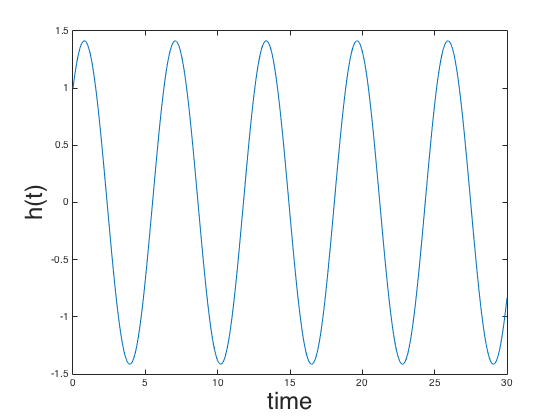
\includegraphics[width=0.15\textwidth, height=0.04\paperheight]{osc_impulse} \end{tabular}};
        \end{scope}

        \begin{scope}[>={Stealth[black]},
                      every node/.style={fill=white,circle},
                      every edge/.style={draw=black, thick}]
            \path [->] (A) edge[bend left] node {\tiny $-1$} (B);
            \path [->] (B) edge[bend left] node {\tiny $1$} (A); 
            \path[->] (U) edge node {\tiny $1$} (A);
            \path[->] (U) edge node {\tiny $1$} (B);
            \path[->] (A) edge[bend right] node {\tiny $1$} (y);
        \end{scope}
        \begin{scope}[>={Stealth[black]},
                      every edge/.style={draw=black, thick}]
            %\path [->] (A) edge[loop left] node {\tiny $\lambda_{1}$} (A);
            %\path [->] (B) edge[loop left] node {\tiny $\lambda_{2}$} (B);
        \end{scope}

     \end{tikzpicture} &
   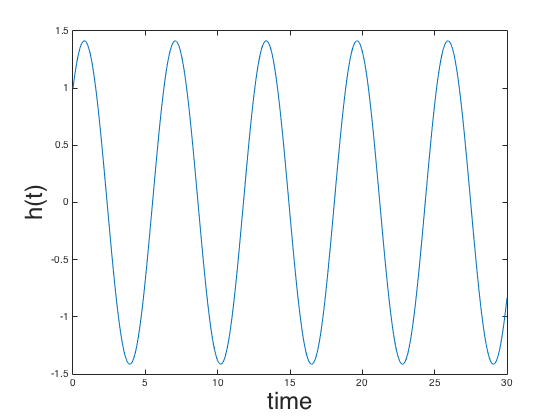
\includegraphics[width=0.5\textwidth, height=0.125\paperheight]{osc_impulse}
\end{tabular}
%  \end{center}
  \caption{
    (Left) 
    Diagram of the gene network in Example \ref{ex:oscillator}
  , and (right) plot of the phenotype $\phi(t)$ against time $t$
  .} \label{fig:oscillator}
\end{figure}


\subsection*{Equivalent gene networks}

As reviewed above,
some systems with identical phenotypes are known to differ, sometimes substantially, at the molecular level; 
systems with identical phenotypes do not necessarily have identical kryptotypes.
How many different mechanisms perform the same function? 

Two systems are equivalent if they produce the same phenotype given the same input,
i.e., have the same input--output relationship.
We say that
the systems defined by $(A,B,C)$ and $(\bar A,\bar B,\bar C)$ are
\textbf{phenotypically equivalent} 
if their impulse response functions are the same:
$h(t) = \bar h(t)$ for all $t \ge 0$.
This implies that for any acceptable input $u(t)$,
if $(\kappa_u(t),\phi_u(t))$ and $(\bar \kappa_u(t),\bar \phi_u(t))$ are the solutions to equation \eqref{eqn:system}
of these two systems, respectively, then
\begin{align*}
      \phi_u(t) = \bar \phi_u(t) \qquad \text{for all} \; t \ge 0.
\end{align*}
% (recall that $\kappa(0) = \bar \kappa(0) = 0$). 
In other words, phenotypically equivalent systems respond identically for \emph{any} input.

One way to find other systems phenotypically equivalent to a given one
is by change of coordinates:
if $V$ is an invertible matrix, then the systems $(A,B,C)$ and $(VAV^{-1},VB,CV^{-1})$
are phenotypically equivalent because their impulse response functions are equal:
  \begin{equation}
    \begin{aligned}
      h(t) &= C e^{A t} B 
      = C V^{-1} V e^{A t} V^{-1} V B \\
      &= C V^{-1} e^{V A V^{-1} t} V B 
      = \bar{C} e^{\bar{A} t} \bar{B} = \bar h(t).
    \end{aligned}
  \end{equation}
These ``changes of coordinates'' are not simply different ways of looking at the same system --
if each dimension of the kryptotype 
corresponds to the concentration of a particular transcription factor,
changing $A$ corresponds to changing the strengths of regulatory interactions.
We will even see below that interactions may change sign. \revpoint{1}{13}
However, not all phenotypically equivalent systems are of this form:
systems can have identical impulse responses without being coordinate changes of each other.
In fact, systems with identical impulse responses can involve interactions between different
numbers of molecules, and thus 
have kryptotypes in
different dimensions altogether.

This implies that most systems have at least $n^2$ degrees of freedom,
where recall $n$ is the number of components of the kryptotype vector.
This is because for an arbitrary $n \times n$ matrix $Z$,
taking $V$ to be the identity matrix plus a small perturbation in the direction of $Z$
above implies that
moving $A$ in the direction of $ZA - AZ$
% (e.g., $\bar A = A + \epsilon(ZA-AZ)$)
while also moving $B$ in the direction of $ZB$ 
and $C$ in the direction of $-CZ$
will leave the phenotype unchanged to second order in the size of the perturbation.
%% I believe the following is necessary and sufficient:
If the columns of $B$ and the rows of $C$ are not all eigenvectors of $A$,
then any such $Z$ will result in a different system.

It turns out that in general, there are more degrees of freedom,
except if the system is \emph{minimal} -- meaning, informally, that it uses the smallest possible number of components
to achieve the desired dynamics.
Results in system theory show that any system can be realized in a particular minimal dimension
(the dimension of the kryptotype, $n_\text{min}$),
and that any two phenotypically equivalent systems of dimension $n_\text{min}$ are related by a change of coordinates.
Since gene networks can grow or shrink following gene duplications and deletions, 
these additional degrees of freedom can apply, in principle, to any system.

Even if the system is not minimal, results from systems theory % -- the Kalman decomposition --
explicitly describe the set of all phenotypically equivalent systems.
% Could define script S here for 'system' if we want: $\Sys$
We refer to $\allS(A_0,B_0,C_0)$ as the set of all systems phenotypically equivalent
to the system defined by $(A_0, B_0, C_0)$:
\begin{equation} \label{eqn:equivalence}
  \begin{aligned}
    \allS(A_0, B_0, C_0) 
      &= \left\{
        (A,B,C) : C e^{At} B = C_0 e^{A_0 t} B_0 \; \text{for}\; t \ge 0 
      \right\}  .
  \end{aligned}
\end{equation}
These systems need not have the same kryptotypic dimension $n$,
but must have the same input and output dimensions ($\ell$ and $m$, respectively).

The Kalman decomposition, which we now describe informally, elegantly characterizes this set
\citep{kalman1963mathematical,kalman1969topics,anderson1966equivalence}.
To motivate this, first note that the input $u(t)$ only directly pushes the system
in certain directions (those lying in the span of the columns of $B$).
As a result, different combinations of input can 
move the system in any direction that lies in what is known as the \emph{reachable subspace}.
Analogously, we can only observe motion of the system in certain directions
(those lying in the span of the rows of $C$),
and so can only infer motion in what is known as the \emph{observable subspace}.
The Kalman decomposition then classifies each direction in kryptotype space
as either reachable or unreachable, and as either observable or unobservable.
Only the components that are both reachable and observable determine the system's phenotype --
that is, components that both respond to an input and produce an observable output. 
% it is possible to add components that respond to an input, 
% but do not influence the output, or components that, in principle, influence the output, but do not respond to any inputs. 

Concretely, the \textbf{Kalman decomposition} of a system $(A,B,C)$  
gives a change of basis $P$ such that
the transformed system $(PAP^{-1},PB,CP^{-1})$
can be written in block matrix form:
\begin{align*}
       PAP^{-1}
       &=
       \left[ \begin{array}{cccc}
           A_{\rno} & A_{\rno,\ro} & A_{\rno,\nrno} & A_{\rno,\nro} \\
           0 & A_{\ro} & 0 & A_{\ro,\nro} \\
           0 & 0 & A_{\nrno} & A_{\nrno,\nro} \\
          0 & 0 & 0 & A_{\nro}
       \end{array} \right] ,
\end{align*}
and
\begin{align*}
     PB
     &=
    \left[ \begin{array}{cccc}
         B_{\rno} \\
         B_{\ro} \\
         0 \\
         0 
   \end{array} \right] 
   &
   (CP^{-1})^T
   &=
   \left[ \begin{array}{cccc}
       0 \\
       C_{\ro}^T \\
       0 \\
       C_{\nro}^T
   \end{array} \right] .
\end{align*}
The $n$-dimensional system has been divided into subspaces
of dimensions $n_\rno + n_\ro + n_\nrno + n_\nro = n$,
and so, for instance, $A_{\rno}$ is the $n_\rno \times n_\rno$ square matrix 
in the top left corner of $P A P^{-1}$. \revpoint{1}{15}
The impulse response of the system is given by
\begin{align*}
      h(t) = C_{\ro} e^{A_{\ro} t} B_{\ro},
\end{align*}
and therefore, the system is phenotypically equivalent to the \emph{minimal} system $(A_{\ro}, B_{\ro}, C_{\ro})$.

This decomposition is unique up to a change of basis that preserves the block structure.
In particular, 
the minimal subsystem obtained by the Kalman decomposition
is unique up to a change of coordinates.
This implies that there is no equivalent system with a smaller number of kryptotypic dimensions
than the dimension of the minimal system.
It is remarkable that the gene regulatory network architecture to achieve a given input--output map is never unique --
both the change of basis used to obtain the decomposition
and, once in this form, all submatrices other than $A_{\ro}$, $B_{\ro}$, and $C_{\ro}$ can be changed without affecting the phenotype,
and so represent degrees of freedom.
(However, some of these subspaces may affect how the system deals with noise.)

\emph{Note on implementation:}
The \emph{reachable subspace},
which we denote by $\reachable$,
is defined to be the closure of $\spn(B)$ under applying $A$
(or equivalently, the span of $B, AB, A^2B, \ldots A^{n-1}B$), \revpoint{AE}{6}
% Analogously to this, we define
and the \emph{unobservable subspace}, 
%$\mathcal{O}$, is the closure of $\spn(C^T)$ under applying $A$.
denoted $\unobservable$, is the largest $A$-invariant subspace
contained in the null space of $C$.
% and $\reachable$ is the largest $A$-invariant subspace contained in the image of $B$.)
The four subspaces, $\rno$, $\ro$, $\nrno$, and $\nro$
are defined from these by intersections and orthogonal complements --
$\ro$ refers to the both \emph{reachable and observable} subspace,
while $\nrno$ refers to the \emph{unreachable and unobservable} subspace,
and similarly for $\nro$ and $\rno$.

%Usually, the dimension $n$ and the reference system $\Sys_0$ is implicit and we write only $\calA$.
%Further, we refer to the set of all linear systems with impulse response $h(t)$, regardless of dimension, to be $\allS$,
%  \begin{align}
%    \allS := \bigcup_{n=\min}^{\infty} \calA_n(\Sys_0)
%  \end{align}

For the remainder of the paper, we interpret $\allS$ as the neutral set in the fitness landscape, 
along which a large population will drift under environmental and selective stasis. 
Even if the phenotype is constrained and remains constant through evolutionary time, 
the molecular mechanism underpinning it is not constrained and likely will not be conserved.

Finally, note that if $B$ and $C$ are held constant --
i.e., if the relationships between environment, kryptotype, and phenotype do not change --
there are \emph{still} usually degrees of freedom. 
The following example \ref{ex:all_osc} gives the set of minimal systems equivalent to the oscillator of Example \ref{ex:oscillator},
that all share common $B$ and $C$ matrices.
The oscillator can also be equivalently realized by a three-gene (or larger) network, and will have even more evolutionary degrees of freedom available, 
as in Figure \ref{fig:3D_osc}.

\begin{example}[All equivalent rewirings of the oscillator] \label{ex:all_osc}
The oscillator of example \ref{ex:oscillator} is minimal, and so any equivalent system is a change of coordinates
by an invertible matrix $V$.
If we further require $B$ and $C$ to be invariant then we need $VB=B$ and $CV=C$.
Therefore
the following one-parameter family $(A(\tau), B, C)$ describes the set of all two-gene systems
phenotypically equivalent to the oscillator:
    \begin{align*}
      A(\tau) &= \frac{-1}{\tau+1} \begin{bmatrix} -\tau & -1 \\ 2 \tau(\tau + 1) + 1 &  \tau \end{bmatrix} \ \text{for} \ \tau \neq -1 .
    \end{align*}
The resulting set of systems are depicted in Figure \ref{fig:all_osc}.
\end{example}


\begin{figure}[H]
    \centering
\begin{tabular}{cc}
\begin{tikzpicture}
\begin{scope}[every node/.style={circle,thick,draw}]
  \node (A) at (0,0) {$\kappa_{1}$};
    \node (B) at (4,0) {$\kappa_{2}$};
    \node[shape=rectangle] (U) at (2,2) {input ($u$)};
    \node[shape=rectangle] (y) at (2,-2) {output ($\phi$)};
\end{scope}

\begin{scope}[>={Stealth[black]},
              every node/.style={fill=white,circle},
              every edge/.style={draw=black, thick}]
    \path [->, sloped] (A) edge[bend left] node {\tiny $-2 \tau - \frac{1}{\tau+1}$} (B);
    \path [->, sloped] (B) edge[bend left] node {\tiny $\frac{1}{\tau+1}$} (A); 
    \path[->] (U) edge node {\tiny $1$} (A);
    \path[->] (U) edge node {\tiny $1$} (B);
    \path[->] (A) edge[bend right] node {\tiny $1$} (y);
\end{scope}
\begin{scope}[>={Stealth[black]},
              every edge/.style={draw=black, thick}]
    \path [->] (A) edge[loop left] node[left] {\tiny $\frac{\tau}{\tau+1}$} (A);
    \path [->] (B) edge[loop right] node[right] {\tiny $\frac{-\tau}{\tau+1}$} (B);
\end{scope}
\end{tikzpicture} &	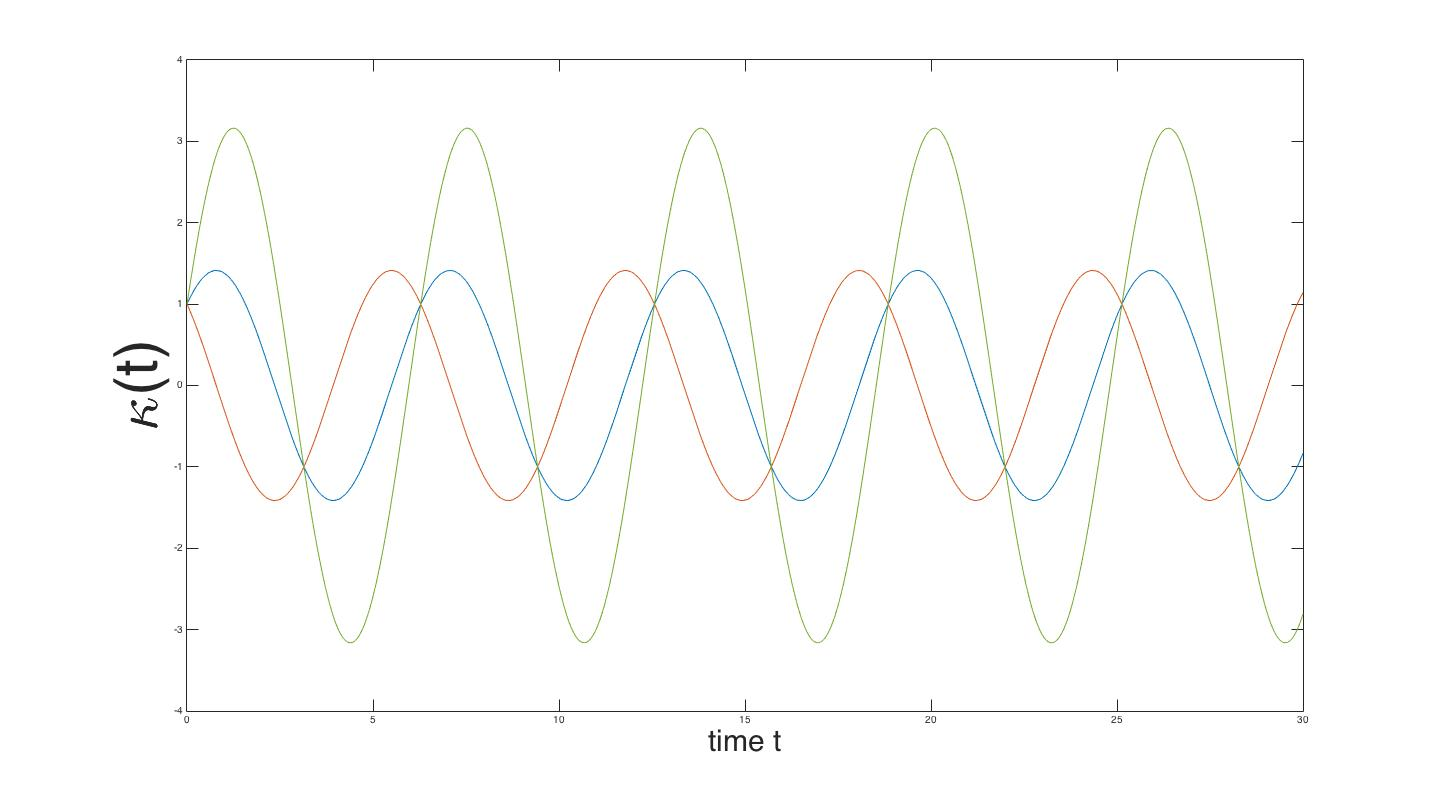
\includegraphics[width=0.5\textwidth, height=0.125\paperheight]{figures/osc_kryp_compare}
    \end{tabular}
% \caption{}
      \caption{
      (Left) $A(\tau)$, the set of all phenotype-equivalent cell cycle control networks.
      (Right) Gene-1 dynamics (blue) for both systems $A(0)$ and $A(-2)$ are identical, however, $A(0)$ gene-2 dynamics (orange) differ from $A(-2)$ (green).
      % Both gene-1 dynamics are given by $\kappa_{1}(t) = \sin t + \cos t$, and gene-2 by $\kappa_{2}(t) = \cos t - \sin t$ ($A(0)$) and $\kappa'_{2}(t) = \cos t + 3 \sin t$ ($A(2)$).
      } 
    \label{fig:all_osc}
\end{figure}

\revpoint{AE}{7}

\begin{figure}[H]
    \begin{center}
\begin{tikzpicture}
\begin{scope}[every node/.style={circle,thick,draw}]
  \node (A) at (0,0) {$\kappa_{1}$};
    \node (B) at (0,4) {$\kappa_{2}$};
    \node (C) at (3.464,2) {$\kappa_{3}$};
    \node[shape=rectangle, rotate=0] (U) at (-2.5,2) {input ($u$)};
    \node[shape=rectangle] (y) at (3.464,0) {output ($\phi$)};
\end{scope}

\begin{scope}[>={Stealth[black]},
              every node/.style={fill=white,circle},
              every edge/.style={draw=black, thick}]
    \path [->, sloped] (A) edge[bend left] node {\tiny $2.2$} (B);
   % \path [->, sloped] (B) edge[bend left] node {\tiny ?} (A); 
    \path [->, sloped] (A) edge[bend right] node {\tiny $2$} (C); 
    %\path [->, sloped] (B) edge[bend right] node {\tiny ?} (C); 
    \path [->, sloped] (C) edge[bend right] node {\tiny $-1$} (A); 
    \path [->, sloped] (C) edge[bend right] node {\tiny $-2.2$} (B); 
    \path[->] (U) edge node {\tiny $1$} (A);
    \path[->] (U) edge node {\tiny $1$} (B);
    \path[->] (A) edge node {\tiny $1$} (y);
\end{scope}
\begin{scope}[>={Stealth[black]},
              every edge/.style={draw=black, thick}]
    \path [->] (A) edge[loop below] node[sloped, below] {\tiny $1$} (A);
    \path [->] (B) edge[loop above] node[sloped, above] {\tiny $1$} (B);
    \path [->] (C) edge[loop right] node[sloped, above] {\tiny $-1$} (C);
\end{scope}
\end{tikzpicture}
  \caption{A possible non-minimal three-gene oscillator, phenotypically equivalent to $A(\tau)$, the systems in Examples \ref{ex:oscillator} and \ref{ex:all_osc}.}
  \label{fig:3D_osc}
\end{center}
\end{figure}

\paragraph{Sexual reproduction and recombination}
Parents with phenotypically equivalent yet differently wired gene networks may produce offspring with dramatically different phenotypes. 
If the phenotypes are significantly divergent then the offspring may be inviable or otherwise dysfunctional, 
despite both parents being well adapted. 
If this is consistent for the entire population, we would consider them to be separate species, in accord with the biological species concept \citep{mayr2000biological}.

First, we must specify how sexual reproduction acts on these systems.
Suppose that each of a diploid organisms' two genomes encodes a set of system coefficients
with the same kryptotype dimension. \revpoint{2}{1}
We assume that a diploid which has inherited systems $(A', B', C')$ and $(A'', B'', C'')$ from its two parents
has phenotype determined by the system that averages these two,
$((A'+A'')/2, (B'+B'')/2, (C'+C'')/2)$.

Each genome an organism inherits is generated by meiosis,
in which both of its diploid parents recombine their two genomes,
and so an $F_1$ offspring carries one system copy from each parent,
and an $F_2$ is an offspring of two independently formed $F_1$s.
If the parents are from distinct populations,
these are simply first-- and second--generation hybrids, respectively.

Exactly how the coefficients 
(i.e., entries of $A$, $B$ and $C$)
of a haploid system inherited by an offspring from her diploid parent
are determined by the parent's two systems
depends on the genetic basis of any variation in the coefficients.
Thanks to the randomness of meiotic segregation,
the result is random to the extent that each parent is heterozygous
for alleles that affect the coefficients.
Since the $i^\text{th}$ row of $A$ summarizes how each gene regulates gene $i$,
and hence is determined by the promoter region of gene $i$,
the elements of a row of $A$ tend to be inherited together,
which will create covariance between entries of the same row.
It is, however, a quite general observation that the variation seen among recombinant systems
is proportional to the difference between the two parental systems.
% This is certainly true if each coefficient is determined by a single nonrecombining locus,
% so that each coefficient in the system produced by meiosis is an independent random choice
% between the two parental coefficients.
% On the other hand, if a coefficient is determined by additive contributions of independently segregating loci,
% then the law of total variance applied after conditioning on the parental origin of each allele
% implies that the variance is equal to one-quarter of the squared difference between parental coefficients.

Offspring formed from two phenotypically identical systems do not necessarily exhibit the same phenotype as both of its parents 
-- in other words $\allS$, the set of all systems phenotypically equivalent to a given one, is not, in general, closed under averaging or recombination.
If sexual recombination among systems drawn from $\allS$ yields systems with divergent phenotypes, 
populations containing significant diversity in $\allS$ can carry genetic load, and isolated populations may fail to produce hybrids with viable phenotypes.


\begin{figure}[H]
\centering
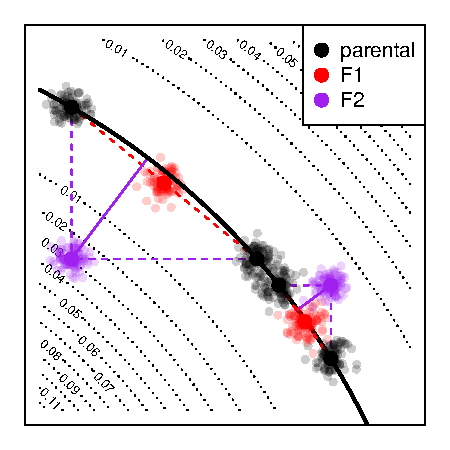
\includegraphics{figures/conceptual_fig}
\caption{
    \label{fig:conceptual_fig}
    A conceptual figure of the fitness consequences of hybridization:
    axes represent system coefficients (i.e., entries of $A$);
    the line of optimal system coefficients is down in black;
    solid lines give phenotypic distances to the optimum.
    A pair of parental populations are shown in black, along the optimum;
    a hypothetical population of $F_1$s are shown in red,
    and the distribution of $F_2$s is shown in purple.
    The two figures differ in the genetic basis, and hence,
    the distribution of $F_2$ phenotypes:
    \textbf{(left)}
    $F_2$s compose all four mixed homozygotes if variation at both
    traits has a simple, one-locus genetic basis in both popualtions; and
    \textbf{(right)}
    $F_2$ show a much wider distribution of phenotypes
    if the genetic basis of variation in each population is polygenic.
}
\end{figure}

\subsection*{Hybrid incompatibility}
Two parents with the optimal phenotype can produce offspring whose phenotype is suboptimal
if the parents have different underlying systems.
How quickly do hybrid phenotypes break down as genetic distance between parents increases?
We will quantify how far a system's phenotype is from optimal
using a weighted difference between impulse response functions.
Suppose that $\rho(t)$ is a nonnegative weighting function, \revpoint{2}{3}
$h_0(t)$ is the \emph{optimal} impulse response function
and define the ``distance to optimum'' of another impulse response function
to be
\begin{align}
\label{eqn:distance}
	D(h) = \left( \int_0^\infty \rho(t) \|h(t) - h_0(t)\|^2 dt \right)^{1/2} .
\end{align}
In practice, we take $\rho(t) = \exp(-t/4\pi)$,
so that fitness is determined by the dynamics of the system over a few multiples of $2 \pi$,
but not longer. \revpoint{AE}{8}
Consider reproduction between a parent with system $(A, B, C)$ 
and another displaced by distance $\epsilon$ in the direction $(X,Y,Z)$,
i.e., having  system $(A + \epsilon X, B + \epsilon Y, C + \epsilon Z)$.
We assume both are ``perfectly adapted'' systems, 
i.e., having impulse response function $h_0(t)$,
and their offspring has impulse response function $h_\epsilon(t)$.
A Taylor expansion of $D(h_\epsilon)$ in $\epsilon$ 
is explicitly worked out in Appendix \ref{apx:H_calc}, and \revpoint{2}{4}
shows that the phenotype of an $F_1$ hybrid between these two is at distance proportional to $\epsilon^2$ from optimal,
while $F_2$ hybrids are at distance proportional to $\epsilon$.
This is because an $F_1$ hybrid has one copy of each parental system,
and therefore lies directly between the parental systems (see Figure \ref{fig:conceptual_fig}) --
the parents both lie in $\allS$, which is the valley defined by $D$,
and so their midpoint only differs from optimal due to curvature of $\allS$.
In contrast, an $F_2$ hybrid may be homozygous for one parental type in some coefficients
and homozygous for the other parental type in others;
this means that each coefficient of an $F_2$ may be equal to either one of the parents,
or intermediate between the two;
this means that possible $F_2$ systems may be as far from the optimal set, $\allS$,
as the distance between the parents.
The precise rate at which the phenotype of a hybrid diverges depends on the geometry
of the optimal set $\allS$ relative to segregating genetic variation.
% in Figure \ref{fig:conceptual_fig}, this is depicted as the angle of the black line (the optimal set) with respect to the coordinates.

\begin{example}[Hybrid incompatibility: misregulation due to system drift] \label{ex:hybrid_osc}
Offspring of two equivalent systems from Example \ref{ex:all_osc}
can easily fail to oscillate.
For instance, the $F_1$ offspring between homozygous parents at $\tau=0$ and $\tau=-2$
has phenotype $\phi_{F_1}(t) = e^t$, rather than $\phi(t) = \sin t + \cos t$.
However, the coefficients of these two parental systems differ substantially,
probably more than would be observed between diverging populations.
In figure \ref{fig:hybs} we compare the phenotypes for $F_1$ and $F_2$ hybrids between more similar parents,
and see increasingly divergent phenotypes as the difference between the parental systems increases.
(In this example, the coefficients of $A(\epsilon)$ differ from those of $A(0)$ by an average factor of $1+\epsilon/2$;
such small differences could plausibly be caused by changes to promoter sequences.)
This divergence is quantified in Figure \ref{fig:osc_incompat},
which shows that mean distance to optimum phenotype of the $F_1$ and $F_2$ hybrid offspring between $A(0)$ and $A(\epsilon)$
increases with $\epsilon^2$ and $\epsilon$, respectively.


\begin{figure}[H]
  \centering
 % \begin{tabular}{ccc}
 %   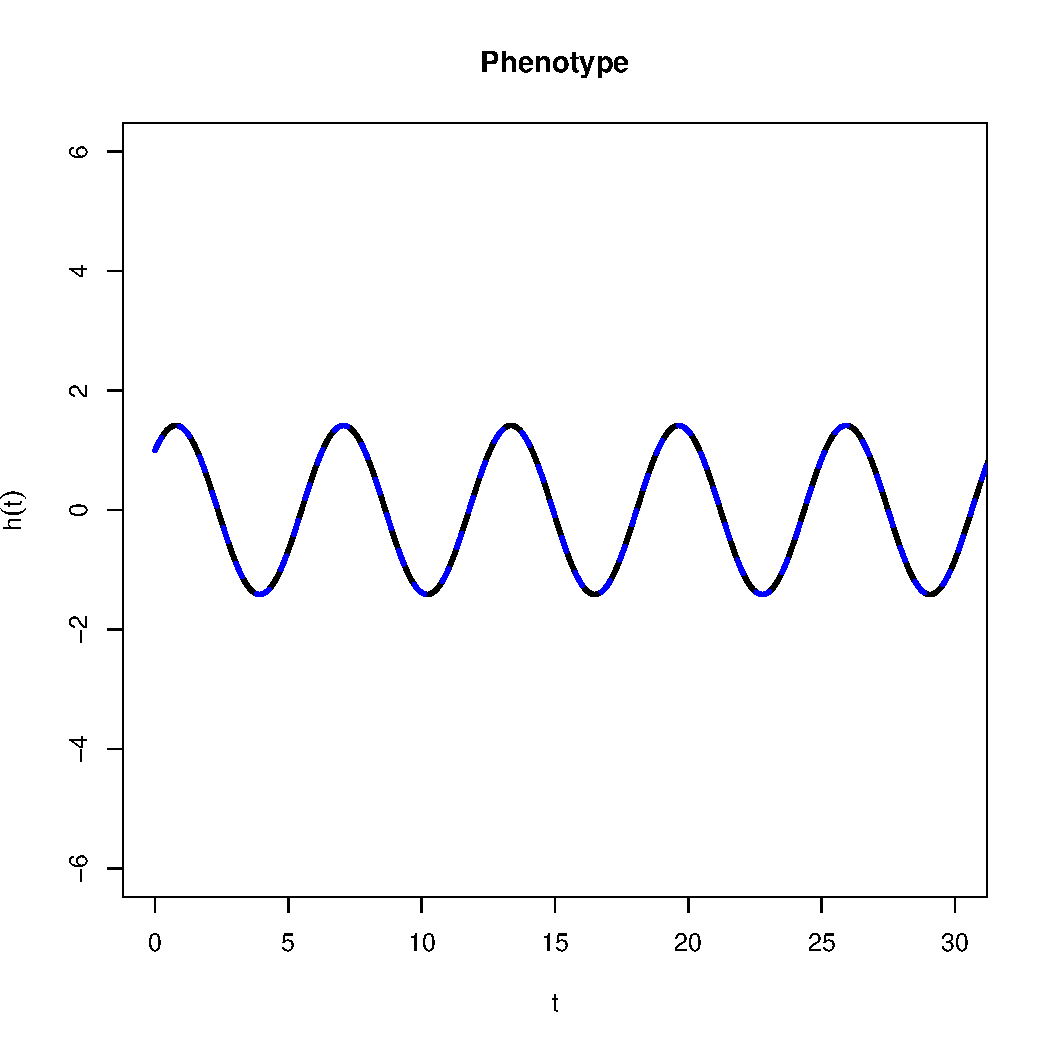
\includegraphics[width=0.5\textwidth, height=0.125\paperheight]{examples/osc_F1_hundreth_tau0} &
 %     \includegraphics[width=0.5\textwidth, height=0.125\paperheight]{examples/osc_F2_hundrethtau0} \\
 %     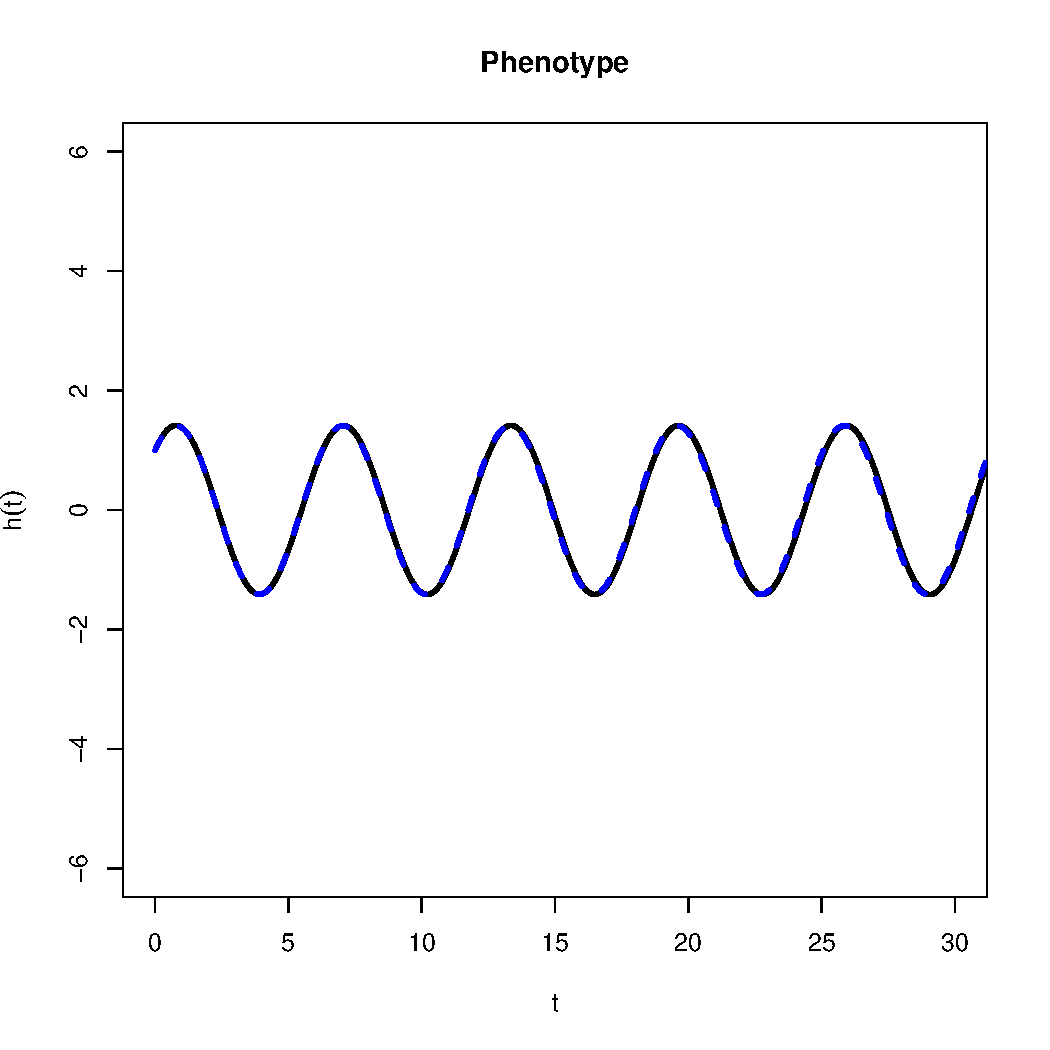
\includegraphics[width=0.5\textwidth, height=0.125\paperheight]{examples/osc_F1_tenth_tau0.pdf} &
 %     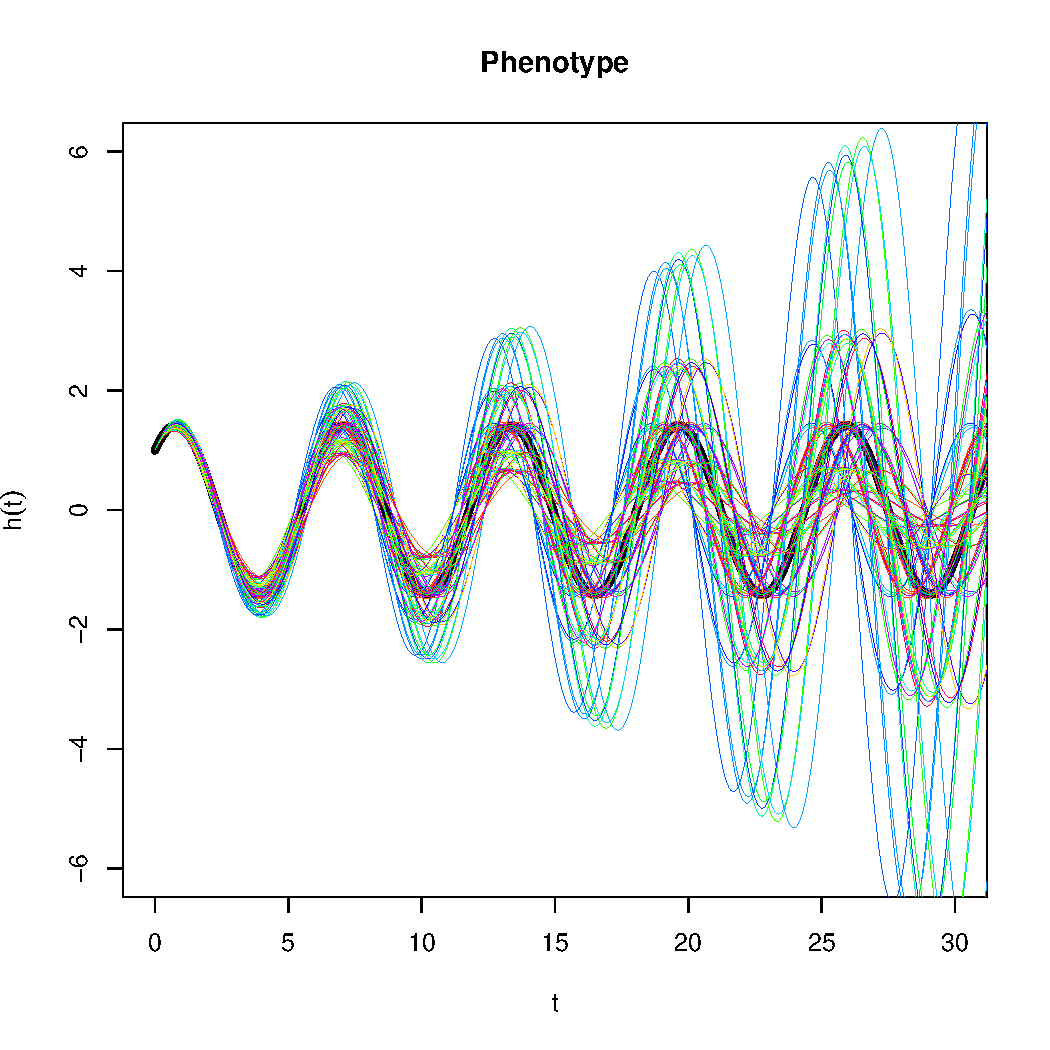
\includegraphics[width=0.5\textwidth, height=0.125\paperheight]{examples/osc_F2_tenthtau0.pdf} \\
 %     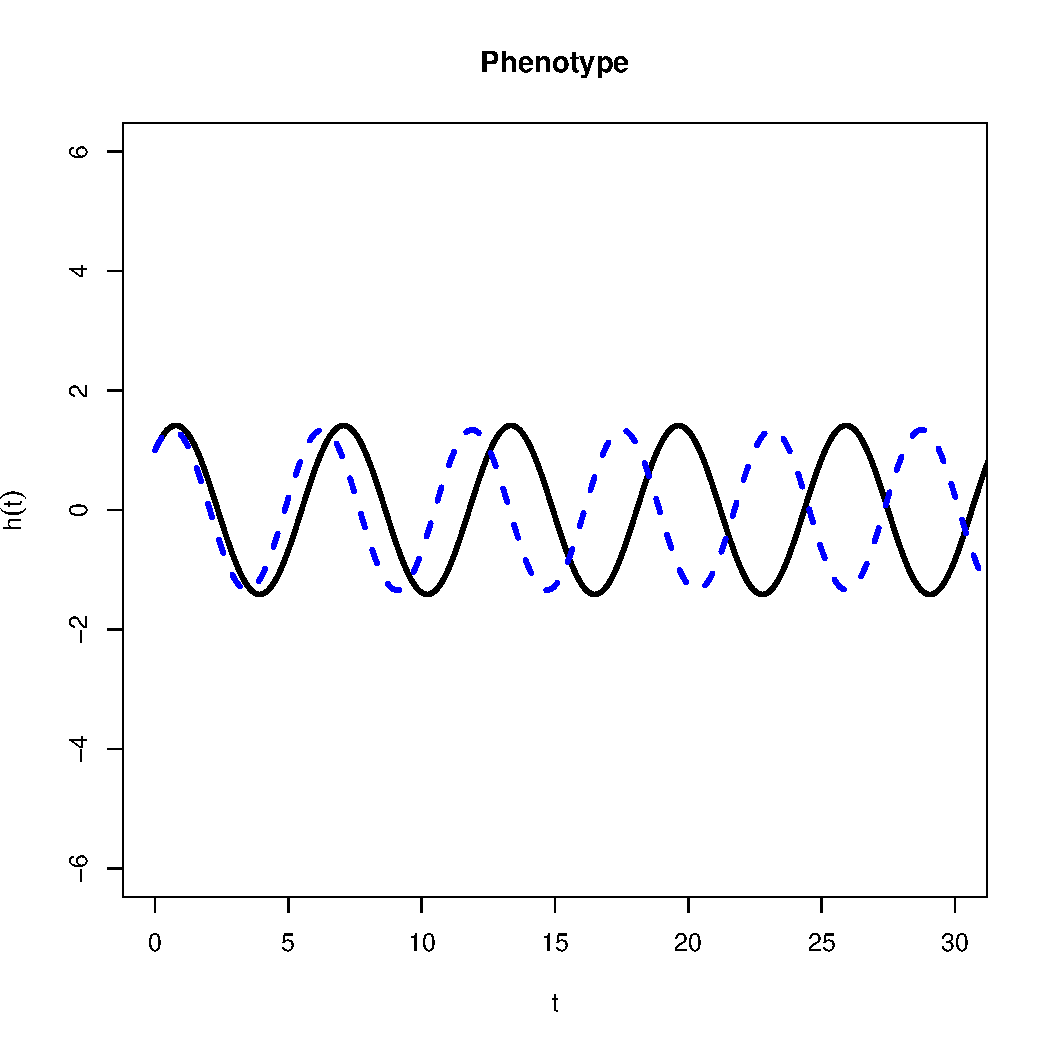
\includegraphics[width=0.5\textwidth, height=0.125\paperheight]{examples/osc_F1_half_tau0.pdf} &
 %     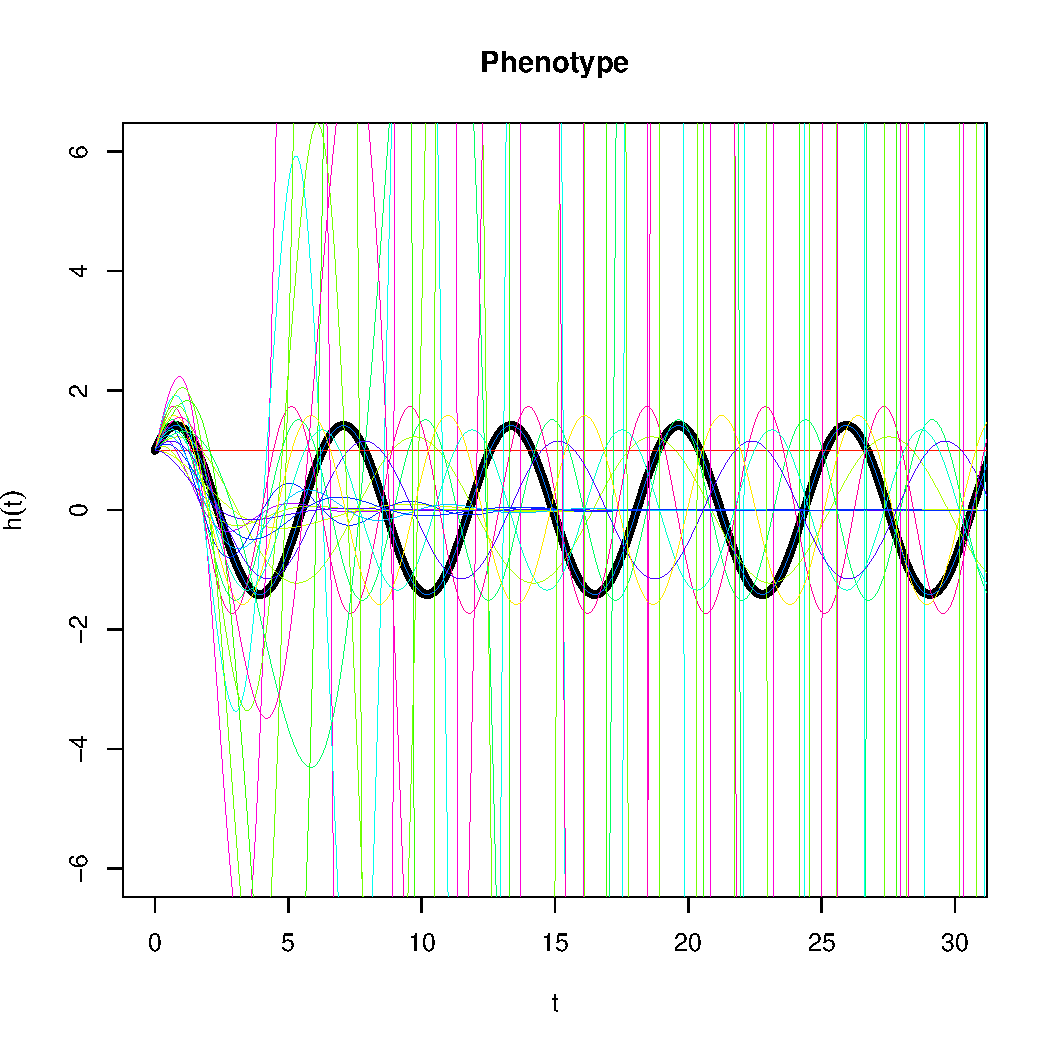
\includegraphics[width=0.5\textwidth, height=0.125\paperheight]{examples/osc_F2_halftau0.pdf}
 % \end{tabular}
  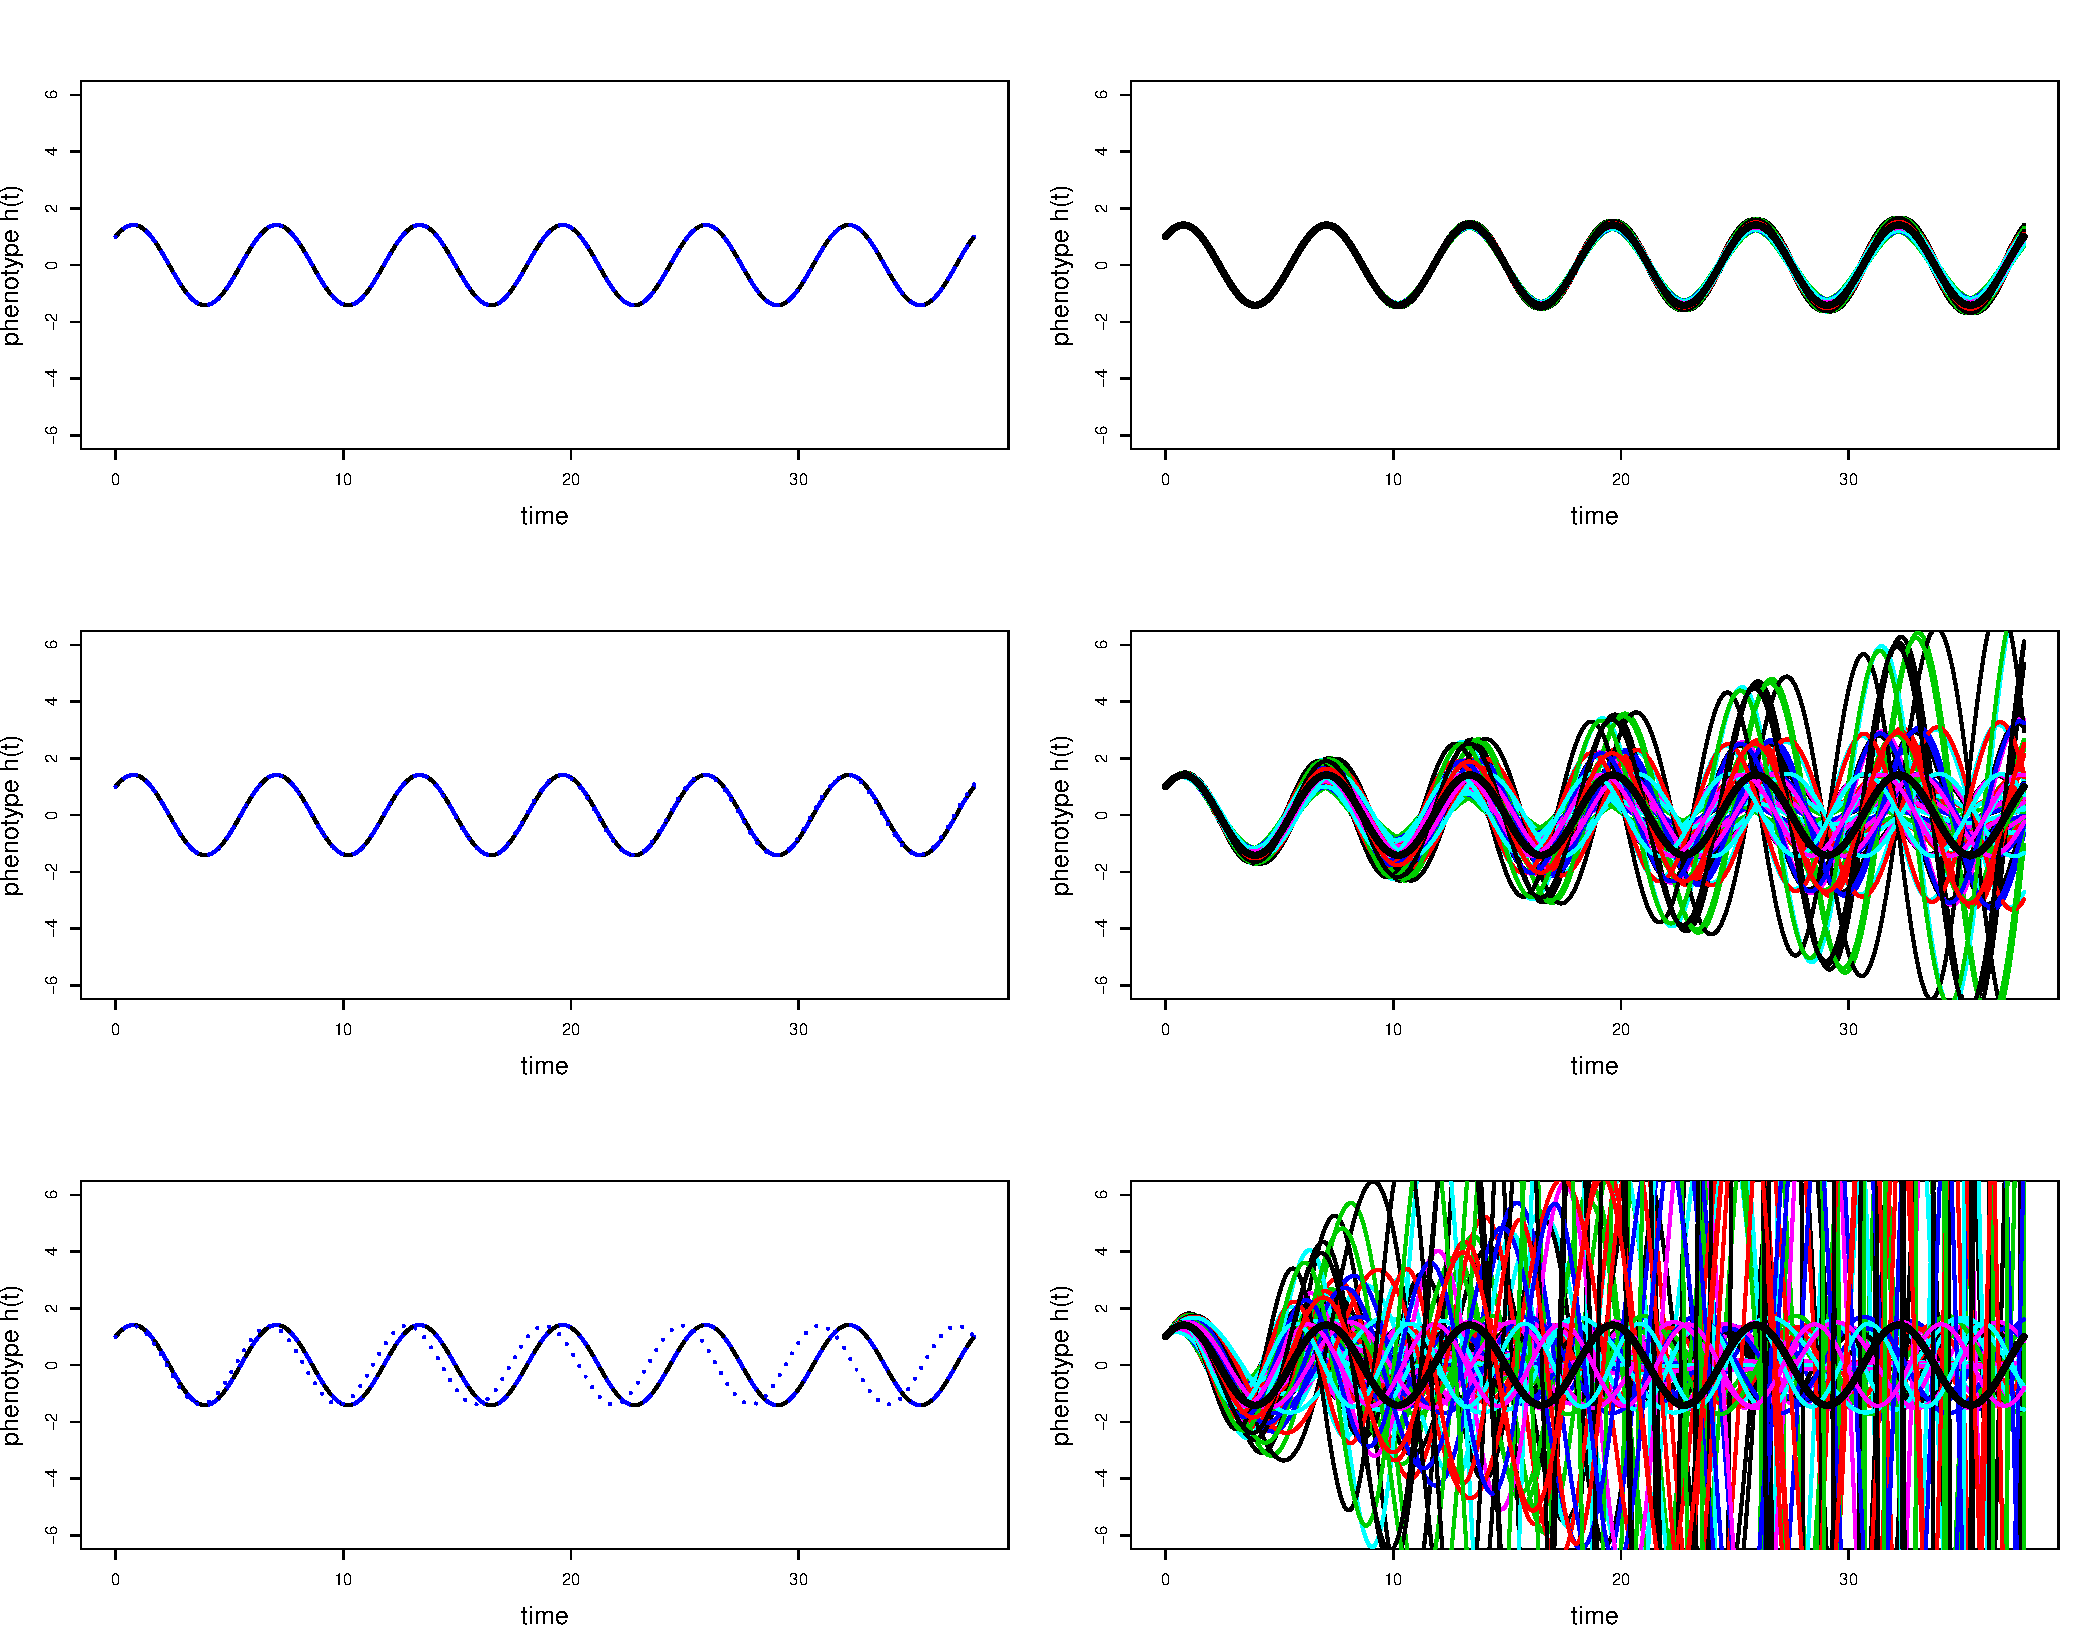
\includegraphics[scale=0.5]{examples/f1f2_newplot}
  \caption{
    \textbf{(left)} Phenotypes of $F_1$ hybrids between a homozygous $A(0)$ parent and, 
    top-to-bottom, homozygous $A(\sfrac{1}{100})$, $A(\sfrac{1}{10})$, and $A(\sfrac{1}{2})$ parents;
    parental coefficients differ by around 0.5\%, 5\%, and 25\% respectively.
    Parental phenotypes ($\sin t + \cos t$) are shown in solid black, and hybrid phenotypes in dashed blue.
    \textbf{(right)} Phenotypes of all $3^4 = 81$ possible $F_2$ hybrids between the same set of parents,
    with parental phenotype again in black.
    %% PLR: There are at most 128 possible F2s, not 256; but many are equivalent; 
    %%   it only matters if the offspring is homo/het/homozygous, so there are 3^4 = 81 possible expression patterns.
    Different colored lines correspond to different $F_2$ hybrids;
    note that some completely fail to oscillate.
  } \label{fig:hybs}
\end{figure}

  \begin{figure}[H]
    \centering
    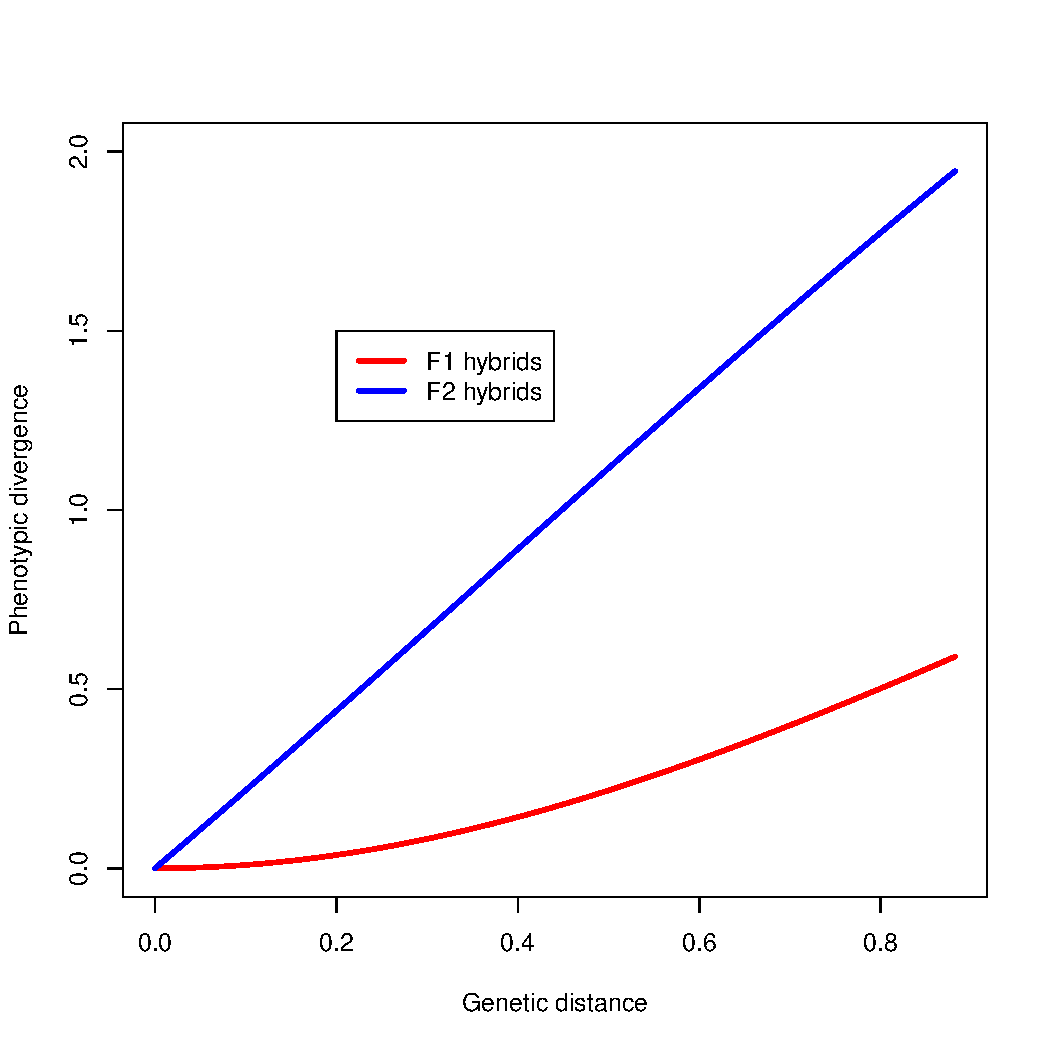
\includegraphics[width=0.5\textwidth]{examples/F2_vs_F1_divergence_tau0}
    \caption{Mean hybrid phenotypic distance from optimum computed with equation \eqref{eqn:distance}, using $\rho(t) = \exp(-t/4\pi)$
    for $F_1$ (black) and $F_2$ (blue) hybrids between $A(0)$ and $A(\epsilon)$ parent oscillators. Genetic distance is computed as 
    $\left(\sum_{ij} (A_{ij}(0) - A_{ij}(\epsilon))^2\right)^{1/2}$.
    }
    \label{fig:osc_incompat}
  \end{figure}
\end{example}

\paragraph{Haldane's rule}
This model naturally predicts
Haldane's rule, the observation that if only one hybrid sex is sterile or inviable 
it is likely the heterogametic sex (e.g., the male in XY sex determination systems) \citep{haldane1922sex, orr1997haldane}.
For example, consider an XY species with a two-gene network where the first gene resides on an autosome and the second gene on the X chromosome.
A male whose pair of haplotypes is 
$\left( \left[ \begin{smallmatrix} A_1 & A_2 \\ \cdot & \cdot \end{smallmatrix} \right], \left[ \begin{smallmatrix} A_1 & A_2 \\ X_1 & X_2 \end{smallmatrix} \right] \right)$
has phenotype determined by $A = \left[ \begin{smallmatrix} A_1 & A_2 \\ X_1 & X_2 \end{smallmatrix} \right]$, 
  if dosage compensation upregulates heterogametes by a factor of two relative to homogametes (as with \emph{Drosophila}),
while a female homozygous for the haplotype
$\left[\begin{smallmatrix} \bar A_1 & \bar A_2 \\ \bar X_1 & \bar X_2 \end{smallmatrix}\right]$, has phenotype determined by
$A = \left[\begin{smallmatrix} \bar A_1 & \bar A_2 \\ \bar X_1 & \bar X_2 \end{smallmatrix}\right]$.
An $F_1$ male offspring of these two will have its phenotype determined by
$\left[\begin{smallmatrix} (A_1 + \bar A_1)/2 & (A_2 + \bar A_2)/2 \\ \bar X_1 & \bar X_2 \end{smallmatrix}\right]$.
If both genes resided on the autosomes, this system would only be possible in an $F_2$ cross.
More generally, 
if the regulatory coefficients for a system are shared between the sex and one or more autosomal chromosomes, 
$F_1$ males are effectively equivalent to purely autosomal-system $F_2$ hybrids, and recall that $F_2$s are significantly less fit on average than $F_1$s (see Figure \ref{fig:osc_incompat}).
Although many alleles will be dominant if the phenotype--fitness relationship is convex,
the underlying mechanism does not depend on the \emph{dominance theory} \citep{turelli1995dominance} to explain Haldane's rule:
instead, it derives from the nature of segregation variance.
% In this setting, Haldane's rule is mechanistically similar to \emph{hybrid breakdown}, 
% the observation that $F_2$ hybrids will often be less fit than $F_1$ hybrid crosses, in the early stages of speciation.
% This mechanism relies on the genetic variation of a system being shared across the sex chromosomes and the autosomes,
% and appears to be consistent with the ``dominance'' theory \citep{orr1997haldane, coyne1998evolutionary, turelli1995dominance} which is often invoked to explain Haldane's rule.
% \plr{Explain that the effects on fitness are dominant.}
%and makes several different predictions than the dominance theory as formulated by \citet{turelli1995dominance}.
%\plr{what are they?}
%\citet{turelli1995dominance} employ a population genetic model which strictly requires alleles causing hybrid incompatibility on the X chromosome not to exhibit additive effects, that is the \emph{dominance coefficient} (typically $h$ in classic population genetics) must not be equal to $\frac{1}{2}$. In their model, if alleles are strictly additive, that is neither dominant nor recessive, then male and female $F_1$ hybrids will drop in fitness at the exact same rates, and therefore defy Haldane's rule. 


%%%%%%%%%%%%%%%%%%%%%%%%%%%%%%%%%%%%%
\subsection*{The speed of speciation}

We have shown that system drift can lead to speciation in principle,
but is it rapid enough to be an important factor in practice?
In other words, after what period of time would we expect the fitness of hybrids
between two allopatric populations to be substantially lower than the parentals?
The population mean of an unconstrained quantitative trait
with additive genetic variance $V_G$ in a population with effective size $N_e$
will move in $t$ generations a random amount whose variance is $t V_G / N_e$ \citep{lande1976natural}.
The mean difference between two such populations has twice the variance.
Although this mean difference is along neutral directions,
we would in many cases expect the range of variation among $F_2$s
in \emph{all} directions to be of the same order
as the differences between the populations, 
as depicted in Figure \ref{fig:conceptual_fig}.
This suggests that, naively, two such populations that have been separated for $t$ generations
will produce $F_2$ offspring that differ from optimal by an amount proportional to $\sqrt{t V_G / N_e}$.
Since we assume they are at a local fitness optimum, without much loss of generality we can assume
that fitness is locally quadratic, and so $F_2$ fitness decays linearly in time:
proportionally to $t V_G / N_e$ -- fastest in small, diverse populations,
This predicts that we need only wait some multiple of $N_e$ generations
until substantial incompatibility has been accumulated.

It is useful to think in more detail about the assumptions in the rough argument above.
The key aspect is how population differences in neutral directions
(along the fitness ridge)
translate to segregation variance in $F_2$s in selectively constrained directions.
To move the system (the $A$ matrix) a given distance
generally involves moving many individual interaction coefficients (the entries $A_{ij}$).
The movements must be coordinated, for the population to stay near the fitness ridge.
However, mixing elements between systems that have made independent sets of coordinated changes
to remain on the fitness ridge
is unlikely to produce a set of coordinated changes;
and the resulting system could move away from the ridge in almost any direction.


%%%%%%%%%%%%%%%%%%%%%%%%%%%%%%%%%%%%%%%%%%%%%%%%%%%%%%%%%%%%%%%
\subsection*{Genetic variation in empirical regulatory systems}

What is known about the key quantity above, the amount of heritable variation in real regulatory networks?
%These are known at best only roughly \citep{felsenstein1988phylogenies},
%so we aim for order-of-magnitude estimates.
The coefficient $A_{ij}$ from the system \eqref{eqn:system} measures how much the rate of net production of $i$ changes
per change in concentration of $j$.
It is generally thought that regulatory sequence change contributes much more to inter- and intraspecific variation
than does coding sequence change affecting molecular structure \citep{schmidt2010fivevertebrate}.
In the context of transcription factor networks this may be affected 
not only by the binding strength of molecule $j$ to the promoter region of gene $i$
but also the effects of other transcription factors (e.g., cooperativity)
and local chromatin accessibility \citep{stefflova2013cooperativity}.
For this reason, 
the mutational target size for variation in $A_{ij}$ may be much larger than the dozens of base pairs
typically implicated in the handful of binding sites for transcription factor $j$ of a typical promoter region,
and single variants may affect many entries of $\allS$ simultaneously.
% (Recall that although these are best modeled through nonlinear terms,
% by linearizing we essentially consider first-order effects.)
% On the other hand, a diverse set of buffering mechanisms are thought to contribute to phenotypic stability
% in the presence of substantial molecular noise \citep{canalization,buffering},
% suggesting that substantial variation in the micro-scale dynamics we consider here
% may be necessary to produce relevant phenotypic effects downstream.

Variation in binding site occupancy may overestimate variation in $A$,
since it does not capture buffering effects (if for instance only one site of many needs to be occupied for transcription to begin),
and variation in expression level measures changes in steady-state concentration (our $\kappa_i$) rather than the \emph{rate} of change.
Nonetheless, these measures likely give us an idea of the scale of variability.
%\citet{kasowski2010variation} found 
It has been shown that between human individuals, there is differential occupancy in 7.5\%
of binding sites of a transcription factor (p65) \citep{kasowski2010variation}.
%\citet{verlaan2009targeted} showed that 
It has also been inferred that cis-regulatory variation
accounts for around 2--6\% of expression variation in human blood-derived primary cells \citep{verlaan2009targeted}, and
%while \citet{lappalainen2013transcriptome} found 
that human population variation 
explained about 3\% of expression variation \citep{lappalainen2013transcriptome}.
Allele-specific expression is indicative of standing genetic \emph{cis}-regulatory variation;
%\citet{wang2017bayesian} found 
allele-specific expression in 7.2--8.5\% of transcripts of a flycatcher species has been observed \citep{wang2017bayesian}, as well as
%while \citet{tung2015genetic} observed 
allele-specific expression in 23.4\% of genes studied in a baboon species \citep{tung2015genetic}. 
Taken together, this suggests that variation in the entries of $A$
may be on the order of at least a few percent between individuals of a population --
doubtless varying substantially between species and between genes.

%%%%%%%%%%%%%%%%%%%%%%%%
%%%%%%%%%%%%%%%%%%%%%
\section*{Discussion}

%%% OUTLINE
% - Summarize methods and main result on rate of speciation.
% - Consistent with F1/F2 divergence and Haldane's rule
% - What empirical evidence is there that this is actually happening? 
%   * incompats due to misregulation (Noor, Witkopp...)
%   * numerous species that are visually indistinguishable (skinks, ferns)
%   * maybe also ref phylogenetic lit
% - What other evidence could be collected?  Note could be just phenotype not fitness. (cite Matute)
% - Is linearity an important assumption?
% - We know that divergent selection and genetic conflict can easily lead to speciation; we've shown neutral drift can maybe surprisingly easily do so also; but it remains unclear the relative contributions of these. Note that although drift may be weaker in any one network there are lots of networks. Could motivate this with Orr's statement.  Perhaps tie in spandrels.

In this paper, we use tools from linear system theory and quantitative genetics
to study the evolution of a mechanistic model of the genotype-phenotype map, 
in which the phenotype is subject to stabilizing selection.
In so doing, we provide an explicit model of
phenogenetic drift \citep{weiss2000phenogenetic} and developmental system drift \citep{true2001developmental}.
In this context, the Kalman decomposition \citep{kalman1963mathematical}
gives an analytical description of all phenotypically equivalent gene networks.
%It also implies that nearly all systems are nonidentifiable,
%and that, in general, there exist axes of genetic variation unconstrained by natural selection.
This description shows that the space of functionally equivalent network architectures increases with the square of a network's size,
and that this space increases further if networks grow larger than absolutely necessary -- that is use more interacting components than the most efficient potential architectures.
In this framework, even minimal gene network architectures -- efficient architectures that contain only the requisite number of interacting parts,
are not structurally unique with respect to function.
Functionally equivalent architectures are often related by continuous parameter changes, suggesting that equivalent networks might be mutationally connected, 
and that there exist axes of genetic variation unconstrained by natural selection.
The independent movement of separated populations along these axes by genetic drift
can lead to a significant reduction in hybrid viability, and thus precipitate speciation,
at a speed dependent on the effective population size and the amount of genetic variation. 
In this model, at biologically reasonable parameter values,
system drift is a significant -- and possibly rapid -- driver of speciation.
This may be surprising because
hybrid inviability appears as a consequence of recombining different, yet functionally equivalent, mechanisms, and since species are often defined by their unique adaptations or morphologies. 

Consistent with empirical observation of hybrid breakdown (e.g., \citet{plotner2017chlorosis}) and transgressive segregation \citep{transgressive}, 
we see that the fitnesses of $F_2$ hybrids drop at a much faster rate than those of $F_1$s.
% since $F_1$ and $F_2$ phenotypes diverge linearly and at the square root of time relative to parentals, respectively.
%\plr{refer to Turelli here}
% In this model, this is due to recombination shuffling system architectures, leaving the $F_2$ system homozygous for one parent at one particular locus and homozygous for the other parent at another possibly incompatible locus.
Another natural consequence of the model is Haldane's rule,
that if only one $F_1$ hybrid sex is inviable or sterile it is likely to be the heterogametic sex.
This occurs because if the genes underlying a regulatory network are distributed among both autosomes and the sex chromosome, 
then heterogametic $F_1$s show variation (and fitnesses) similar to that seen in $F_2$ hybrids.

Is there evidence that this is actually occurring?
System drift and network rewiring has been inferred across the tree of life \citep{wotton2015quantitative, crombach2016gap, dalal2017transcription, johnson2017rewiring, ali2017quantitative},
and there is often significant regulatory variation segregating within populations.
Transcription in hybrids between closely related species with conserved transcriptional patterns can also be divergent 
\citep{haerty2006gene, maheshwari2012cis, coolon2014tempo, michalak2004association, mack2016gene}, and hybrid incompatibilities have been attributed to cryptic molecular divergence underlying conserved body plans \citep{gavin2013embryonic}. 
Furthermore, in cryptic species complexes (e.g., sun skinks \citep{barley2013challenge}),
%strongly reproductively incompatible species
genetically distinct species
may be nearly morphologically indistinguishable.


\paragraph{The origin of species not by means of natural selection?}
% this is neutral, in contrast to other models. although some folks advocate nonadaptive speciation.
% other mechanisms also probably important
% but this one may be strong since happens in all networks at once
As classically formulated, 
the Dobzhansky-Muller model of hybrid incompatibility is agnostic to the relative importance of neutral versus selective genetic substitutions \citep{coyne1998evolutionary},
and plausible mechanisms have been proposed
whereby Dobzhansky--Muller incompatibilities could originate
under neutral genetic drift \citep{lynch2000origin}
or stabilizing selection \citep{fierst}.
The same holds for the ``pathway model'' \citep{lindtke2015genetic},
which is closer to the situation here.
However, previous authors have argued that neutral processes are likely too slow to be a significant driver of speciation \citep{nei1983models,seehausen2014genomics}.
% Using simulations, \citet{porter2002speciation} demonstrated the accumulation of hybrid incompatibilities under directional, but not stabilizing selection, and \citet{palmer2009dynamics} observed the appearance of incompatibilities in populations evolving in a constant environment, only if the populations were suboptimally adapted.
% In light of the few known incompatibilities, 
This has led some to conclude that hybrid incompatibility is typically a byproduct of positive selection \citep{orr2004speciation, schluter2009evidence} 
or a consequence of genetic conflict \citep{presgraves2010molecular, crespi2013conflictual},
two processes that typically act much more rapidly than genetic drift.
% In contrast, the model we develop here suggests that even under strictly neutral conditions, 
% system drift can lead to speciation, at a rate fast enough 
% to play a substantial role in species formation across the tree of life. 
However, our calculations suggest that even under strictly neutral processes,
hybrid fitness breaks down as a function of genetic distance
rapidly enough to play a substantial role in species formation across the tree of life. 
This is consistent with broad patterns
such as the relationship between molecular divergence and genetic isolation 
% across diverse taxa and ecologies 
seen by \citet{roux2016shedding}, 
and the clocklike speciation rates observed by \citet{hedges2015tree}.
% (as diversification is not observed to be accelerated following mass extinctions).

These explanations are not mutually exclusive.
All of these forces -- adaptive shifts, conflict, and network drift --
are plausible drivers of speciation, and may even interact.
Many of our observations carry over to models of directional selection --
for instance, rapid drift along the set of equivalent systems
could be driven by adaptation in a different, pleiotropically coupled system.
Or, reinforcement due to local adaptation might provide a selective pressure
that speeds up system drift.
Furthermore,
while the fitness consequences of incompatibility in any one given network may be small, 
the cumulative impact of system drift across the many different networks an organism relies on may be substantial. 
It remains to be seen how the relative strengths of these forces compare.

% Of course the basic assumptions of this model will be violated in practice (constant selective pressures, etc.), however, this model can function as a ``neutral null'' description of gene network evolution (a strategy advocated for by \citet{lynch2007frailty, fay2008evaluating, koonin2016splendor}). If this model succeeds in describing actual system evolution, it can be inferred that the mechanism underlying species formation does not require the inclusion of adaptation or changes in selection to explain the emergence of hybrid incompatibility.

% \paragraph{Population isolates and genetic load}
% Above we have mostly discussed the case of two separated populations of equal size.
% In contrast, consider a small subset of a large population that is suddenly isolated.
% It will have a large amount of genetic variance, thanks to its history,
% but a small population size -- and so can drift quite quickly until it exhausts its genetic variation.
% By this point, it could have accumulated substantial incompatibility with the parental population.
% Similarly, in a species with substantial isolation by distance, geographically local systems drift
% might lead to genetic load due only to recombination, much as in \citep{phillips1996maintenance}.

\paragraph{The dimensionality of trait space} \revpoint{1}{8}
We have focused on examples of single traits (where the phenotype is one-dimensional),
but phenotypes under selection are often high-dimensional,
and variation in different traits often share a genetic basis.
However, we still expect many degrees of freedom
as long as there are components of the system not directly and individually constrained by selection
(i.e., a kryptotype). % since if C = I then there's no nontrivial transformations that preserve C
Even in networks where the phenotype and kryptotype are of the same dimension,
system theory shows us that there will always be available degrees of freedom
as specific system realizations are only unique up to a change of coordinates.
Some phenotypes, however, require kryptotypic dimensions to be larger than that of the phenotype.
For instance, many systems have minimal realizations (\emph{e.g.}, the oscillator in Example \ref{ex:all_osc}) where the dimension of the kryptotype is larger
than that of the phenotype, implying that for these phenotypic dynamics to be realized, the kryptotype dimension \emph{has} to be larger than the dimension of the phenotype.
Even if components of the system's internal state are directly subject to selection
and the mode of action of the environment on the internal state is constrained
(so, the input and output matrices $B$ and $C$ are fixed)
then one could still perturb $A$ as described above by $ZA - AZ$
if $ZB$ and $CZ$ are both zero, implying a number of degrees of freedom that still grows with $n^2$
for fixed $\ell$ and $m$.
Generically, the number of degrees of freedom is $n(n - \ell - m)$,
so that in a system of $n$ components, if even one component is not directly constrained,
this leads to $n$ degrees of freedom.
Whatever the true ``dimensionality'' of phenotype space of a typical organism,
there are undoubtedly aspects of its underlying molecular machinery that are not directly constrained,
suggesting large numbers of degrees of freedom.
Note that pleiotropy does not directly affect this argument at all --
indeed, many phenotypically equivalent changes will lead to denser $A$ matrices and hence more pleiotropy.
However, more pleiotropic genes may be more strongly constrained,
making it more difficult for systems to make the required compensatory changes for system drift.
% Whatever it is, however, it seems unlikely 
% that it would approach the dimensionality of kryptotype space,
% which is something related to the number of genes.
% even under universal pleiotropy \citep{universal_pleiotropy, boyle2017expanded},

\paragraph{Nonlinearity and model assumptions}
Of course, real regulatory networks are not linear dynamical systems.
Most notably, physiological limits put upper bounds on expression levels,
implying saturating response curves.
It remains to be seen how well our results carry over into real systems,
but the fact that most nonlinear systems can be locally approximated by a linear one
suggests our qualitative results may hold more generally.
Furthermore, nonidentifiability (which implies the existence of neutral directions)
is often found in practice in moderately complex models of biological systems \citep{gutenkunst2007universally, piazza2008diverse}.

Finally, despite our model's precise separation of phenotype and kryptotype, this relationship in nature may be far more complicated as aspects of the kryptotype may be less ``hidden'' than we currently assume, and the neutral network changes we describe here may only be nearly neutral. For instance, attributes excluded from the phenotype as modeled here ignore the potential energy costs associated with excessively large (non-minimal) kryptotypes, as well as the relationship between a specific network architecture and robustness to mutational, transcriptional, or environmental noise.
% Despite the model's simplifications and potentially nontrivial oversights, it may still roughly reflect and shed light upon speciation patterns as they occur in nature.
More precise modeling will require better mechanistic understanding not only of biological systems,
but also the nature of selective pressures
and genetic variation in these systems.

%Maybe compare to \citet{fierst}?
%
%hominids; neanderthal load.

\section*{Acknowledgements}

    We would like to thank Sergey Nuzhdin, Stevan Arnold, Michael Turelli, Patrick Phillips, Erik Lundgren and Hossein Asgharian for valuable discussion. 
    We would also like to thank Nick Barton, Sarah Signor, Todd Parsons, Joachim Hermisson for very helpful comments on the manuscript.
    Work on this project was supported by funds from
    the Sloan Foundation and the NSF (under DBI-1262645) to PR.



\bibliographystyle{plainnat}
\bibliography{krefs}
%\end{multicols}

\normalsize
\appendix

%%%%%%%%%%%%%%%%%%%%%%%%%%%%%%%
\section{Local expansion of the fitness surface}
\label{apx:H_calc}

Suppose that $\rho(t) \ge 0$ is a weighting function on $[0,\infty)$
so that fitness is a function of $L^2(\rho)$ distance of the impulse response from optimal.
With $h_0(t) = C_0 e^{tA_0} B_0$ a representative of the optimal set:
\begin{equation}
    \begin{aligned}
        D(A, B, C)^2
        &:= 
        \int_0^\infty \rho(t) \left| h_A(t) - h_0(t) \right|^2 dt \\
        &:= 
        \int_0^\infty \rho(t) \left| C e^{At} B - C_0 e^{A_0 t} B_0 \right|^2 dt \\
        &= 
        \int_0^\infty \rho(t) \tr\left\{
            \left( C e^{At} B - C_0 e^{A_0 t} B_0 \right)^T
            \left( C e^{At} B - C_0 e^{A_0 t} B_0 \right)
        \right\} dt \\
        &= 
        \int_0^\infty \rho(t) \tr\left\{
            \left( C e^{At} B - C_0 e^{A_0 t} B_0 \right)
            \left( C e^{At} B - C_0 e^{A_0 t} B_0 \right)^T
        \right\} dt  ,
        % &= 
        % \int_0^\infty \rho(t)  \tr\left\{
        %         C e^{At} B B^T e^{A^T t} C^T 
        %         - C_0 e^{A_0t} B_0 B^T e^{A^T t} C^T 
        %         \right. \\ &\qquad \qquad \left. {}
        %         - C e^{At} B B_0^T e^{A_0^T t} C_0^T 
        %         + C_0 e^{A_0t} B_0 B_0^T e^{A_0^T t} C_0^T 
        % \right\} dt \\
        % \int_0^\infty \rho(t) \left| C \left( e^{At} - e^{A_0 t} \right) B \right|^2 dt \\
        % &= 
        % \int_0^\infty \rho(t) C \left( e^{At} - e^{A_0 t} \right) B B^T \left( e^{At} - e^{A_0 t} \right)^T C^T dt
    \end{aligned}
\end{equation}
where $\tr X$ denotes the trace of a square matrix $X$.
How does this change as we perturb about $(A_0, B_0, C_0)$?
First we differentiate with respect to $A$, keeping $B=B_0$ and $C=C_0$ fixed.
Since
\begin{equation}
  \begin{aligned}
      \frac{d}{du} e^{(A+uZ)t} \vert_{u=0}
      &=
      \int_0^t e^{As} Z e^{A(t-s)} ds, 
  \end{aligned}
\end{equation}
we have that
\begin{equation}
  \begin{aligned}
      \frac{d}{du} D(A+uZ,B_0,C_0)^2 \vert_{u=0}
      &=
        2 \int_0^\infty \rho(t) \tr\left\{ C_0 \left( \int_0^t e^{As} Z e^{A(t-s)} ds \right) B_0 B_0^T \left( e^{At} - e^{A_0 t} \right)^T C_0^T \right\} dt \\
      &=
        2 \int_0^\infty \rho(t) \tr\left\{ C_0 \left( \int_0^t e^{As} Z e^{A(t-s)} ds \right) B_0 \left( h_A(t) - h_0(t) \right)^T \right\} dt 
  \end{aligned}
\end{equation}
and, by differentiating this and supposing that $A$ is on the optimal set,
i.e., $h_A(t)=h_0(t)$, (so without loss of generality, $A=A_0$):
\begin{equation}
  \begin{aligned}
      \calH^{A,A}(Y,Z) 
      &:= 
      \frac{1}{2} \frac{d}{du} \frac{d}{dv} D(A_0+uY+vZ,B_0,C_0)^2 \vert_{u=v=0} \\
      &=
        \int_0^\infty \rho(t) \tr\left\{ C_0 
        \left( \int_0^t e^{A_0 s} Y e^{A_0 (t-s)} ds \right) 
        B_0 B_0^T 
        \left( \int_0^t e^{A_0 s} Z e^{A_0 (t-s)} ds \right)^T
        C_0^T \right\} dt  .
  \end{aligned}
\end{equation}

The function $\calH$ will define a quadratic form.
To illustrate the use of this, suppose that $B$ and $C$ are fixed.
% Here $\calH$ is the quadratic form underlying the Hamiltonian.
By defining $\Delta_{ij}$ to be the matrix with a 1 in the $(i,j)$th slot
and 0 elsewhere,
the coefficients of the quadratic form is
\begin{equation}
    \begin{aligned}
        H_{ij, k\ell}(A)
        &:=
        \calH(\Delta_{ij}, \Delta_{k\ell}) .
    \end{aligned}
\end{equation}

We could use this to get the quadratic approximation to $D$ near the optimal set.
To do so, it'd be nice to have a way to compute the inner integral above.
Suppose that we diagonalize $A = U \Lambda U^{-1}$.
Then
\begin{equation} \label{eqn:exp_deriv}
  \begin{aligned}
      \int_0^t e^{As} Z e^{A(t-s)} ds 
      &=
      \int_0^t U e^{\Lambda s} U^{-1} Z U e^{\Lambda (t-s)} U^{-1} ds 
  \end{aligned}
\end{equation}
Now, notice that
\begin{equation}
  \begin{aligned}
      \int_0^t e^{s \lambda_i} e^{(t-s) \lambda_j} ds
      &=
      \frac{ e^{t \lambda_i} - e^{t \lambda_j} }{ \lambda_i - \lambda_j } 
          \qquad & \text{if} \quad i \neq j \\
      &=
          t e^{t \lambda_i} 
          \qquad & \text{if} \quad i = j 
  \end{aligned}
\end{equation}
Therefore, 
defining
\begin{equation}
    \begin{aligned}
    X_{ij}(t,Z) 
       &= 
        \left( U^{-1} Z U \right)_{ij}
      \frac{ e^{t \lambda_i} - e^{t \lambda_j} }{ \lambda_i - \lambda_j } 
          \qquad & \text{if} \quad i \neq j \\
      &=
          \left( U^{-1} Z U \right)_{ii}
          t e^{t \lambda_i} 
          \qquad & \text{if} \quad i = j 
    \end{aligned}
\end{equation}
moving the $U$ and $U^{-1}$ outside the integral and integrating we get that
\begin{equation}
  \begin{aligned}
      \int_0^t e^{As} Z e^{A(t-s)} ds 
      &=
      U X(t,Z) U^{-1} .
  \end{aligned}
\end{equation}
This implies that
\begin{equation}
    \begin{aligned}
        D(A_0+\epsilon Z)^2
        &\approx \frac{1}{2} \epsilon^2 
        \int_0^\infty
            \rho(t) \tr\left\{ C U X(t,Z) U^{-1} B B^T (U^{-1})^T X(t,Z)^T U^T C^T \right\}
        dt .
    \end{aligned}
\end{equation}

To compute the $n^2 \times n^2$ matrix $H$,
we see that if $Z=\Delta_{k \ell}$, then
\begin{equation}
  \begin{aligned}
      X_{ij}^{k\ell}(t) 
      &= 
      (U^{-1})_{\cdot k} U_{\ell \cdot}
      \frac{ e^{t \lambda_i} - e^{t \lambda_j} }{ \lambda_i - \lambda_j } 
          \qquad & \text{if} \quad i \neq j \\
      &=
      (U^{-1})_{\cdot k} U_{\ell \cdot}
      t e^{t \lambda_i} 
          \qquad & \text{if} \quad i = j 
  \end{aligned}
\end{equation}
where $U_{k \cdot}$ is the $k$th row of $U$,
and so
\begin{equation}
    \begin{aligned}
        H_{ij, k\ell}(A)
        &=
        \int_0^\infty
            \rho(t) \tr\left\{ C U X^{ij}(t) U^{-1} B B^T (U^{-1})^T X^{k\ell}(t)^T U^T C^T \right\}
        dt .
    \end{aligned}
\end{equation}
This implies that
\begin{equation}
    \begin{aligned}
        D(A_0+\epsilon Z)^2
        &\approx \frac{1}{2} \epsilon^2 \sum_{ijk\ell} H_{ij,k\ell}(A_0) Z_{ij} Z_{k\ell}  .
    \end{aligned}
\end{equation}

By section \ref{ss:quant_gen},
if we set $\Sigma=\sigma^2 I$ and $U=H$,
then a population at $A_0+Z$ experiences a restoring force of strength
$(I + \sigma^2 H^{-1})^{-1} Z$ (treating $Z$ as a vector and $H$ as an operator on these).
If $\sigma^2$ is small compared to $H^{-1}$
then this is approximately $-\sigma^2 H^{-1} Z$.
This suggests that the population mean follows an Ornstein-Uhlenbeck process,
as described (in different terms) in \citet{hansen1996translating}.

More generally, $B$ and $C$ may also change.
To extend this we need the remaining second derivatives of $D^2$.
First, in $B$:
\begin{equation}
    \begin{aligned}
        \mathcal{H}^{B,B}(Y,Z)
        &:= 
        \frac{1}{2} \frac{d}{du} \frac{d}{dv} D(A_0,B_0+uY+vZ,C_0)\vert_{u=v=0} \\
        &=
        \frac{1}{2} \int_0^\infty \rho(t) \tr\left\{ 
        C_0 e^{t A_0}
        \frac{d}{du} \frac{d}{dv} 
        (uY+vZ)
        (uY+vZ)^T
        \vert_{u=v=0} 
        e^{t A_0^T} C_0^T 
        \right\} dt  \\
        &=
        \frac{1}{2} \int_0^\infty \rho(t) \tr\left\{ 
        C_0 e^{t A_0}
        \left( Y Z^T + Z Y^T \right)
        e^{t A_0^T} C_0^T 
        \right\} dt  .
  \end{aligned}
\end{equation}
Next, in $C$:
\begin{equation}
    \begin{aligned}
        \mathcal{H}^{B,B}(Y,Z)
        &:= 
        \frac{1}{2} \frac{d}{du} \frac{d}{dv} D(A_0,B_0,C_0+uY+vZ)\vert_{u=v=0} \\
        &=
        \frac{1}{2} \int_0^\infty \rho(t) \tr\left\{ 
        B_0 e^{t A_0^T}
        \frac{d}{du} \frac{d}{dv} 
        (uY+vZ)^T
        (uY+vZ)
        \vert_{u=v=0} 
        e^{t A_0} B_0
        \right\} dt  \\
        &=
        \frac{1}{2} \int_0^\infty \rho(t) \tr\left\{ 
        B_0 e^{t A_0^T}
        \left( Y Z^T + Z Y^T \right)
        e^{t A_0} B_0
        \right\} dt  .
  \end{aligned}
\end{equation}
Now, the mixed derivatives in $B$ and $C$:
\begin{equation}
    \begin{aligned}
        \mathcal{H}^{B,C}(Y,Z)
        &:= 
        \frac{1}{2} \frac{d}{du} \frac{d}{dv} D(A_0,B_0+uY,C_0+vZ)\vert_{u=v=0} \\
        &=
        \int_0^\infty \rho(t) \tr\left\{ 
        Y e^{t A_0^T} C_0^T Z e^{t A_0} B_0
        \right\} dt  .
  \end{aligned}
\end{equation}
In $A$ and $B$
\begin{equation}
    \begin{aligned}
        \mathcal{H}^{A,B}(Y,Z)
        &:= 
        \frac{1}{2} \frac{d}{du} \frac{d}{dv} D(A_0+uY,B_0+vZ,C_0)\vert_{u=v=0} \\
        &=
        \int_0^\infty \rho(t) \tr\left\{ 
        C_0 \left(\int_0^t e^{s A_0} Y e^{(t-s) A_0} ds \right) B_0
        Z^T e^{t A_0} C_0
        \right\} dt  ,
  \end{aligned}
\end{equation}
and finally in $A$ and $C$:
\begin{equation}
    \begin{aligned}
        \mathcal{H}^{A,C}(Y,Z)
        &:= 
        \frac{1}{2} \frac{d}{du} \frac{d}{dv} D(A_0+uY,B_0,C_0+vZ)\vert_{u=v=0} \\
        &=
        \int_0^\infty \rho(t) \tr\left\{ 
        C_0 \left(\int_0^t e^{s A_0} Y e^{(t-s) A_0} ds \right) B_0
        B_0 e^{t A_0} Z
        \right\} dt  .
  \end{aligned}
\end{equation}

Together, numerical computation of these expressions,
along with estimates of genetic covariance within a population,
allow precise predictions of evolutionary dynamics of a particular system.
The approximation should be good as long as the second-order Taylor approximation holds.

% reviews here if toggled above
% \ifsubmission\processdelayedfloats\fi

\includereviews


\end{document}


